\documentclass[conference]{IEEEtran}
% Add the compsoc option for Computer Society conferences.
%
% If IEEEtran.cls has not been installed into the LaTeX system files,
% manually specify the path to it like:
% \documentclass[conference]{../sty/IEEEtran}


% Badges
\usepackage[available,functional,reproduced]{ndssbadges}

\pagestyle{plain}

% *** Do not adjust lengths that control margins, column widths, etc. ***
% *** Do not use packages that alter fonts (such as pslatex).         ***
% There should be no need to do such things with IEEEtran.cls V1.6 and later.
% (Unless specifically asked to do so by the journal or conference you plan
% to submit to, of course. )


% correct bad hyphenation here
%\hyphenation{op-tical net-works semi-conduc-tor}


% Uncomment to enable anonymous submission
%\newcommand*{\ANON}{}%
% Uncomment to make the paper "submission-ready"
\newcommand*{\SUBMISSION}{}%

%  Hide URLs for anonymous submission
\ifdefined\ANON
\newcommand{\repo}{\url{https://www.dropbox.com/sh/v8ct0un8x7loi3m/AAB6op3fOWCp9qKEYlFI_Upba?dl=0}}
\newcommand{\repotamarin}{\textbf{redacted}}
\newcommand{\repoprl}{\textbf{redacted}}
\newcommand{\reposimulation}{\textbf{redacted}}
\else
\newcommand{\repo}{\url{https://github.com/EricssonResearch/v2x-self-revocation}}
\newcommand{\repotamarin}{\url{https://github.com/EricssonResearch/v2x-self-revocation/tree/main/proofs}}
\newcommand{\repoprl}{\url{https://github.com/EricssonResearch/v2x-self-revocation/tree/main/prl}}
\newcommand{\reposimulation}{\url{https://github.com/EricssonResearch/v2x-self-revocation/tree/main/simulation}}
\fi


\ifdefined\SUBMISSION
\usepackage[disable]{todonotes}
\else
\usepackage[textsize=footnotesize]{todonotes}
\presetkeys{todonotes}{fancyline}{}
\setlength{\marginparwidth}{1.3cm}
\setlength{\marginparsep}{3pt}
\fi

\newcommand{\christoph}[1]{\todo[color=orange!20]{\textbf{Christoph:} #1}}
\newcommand{\eddy}[1]{\todo[color=yellow]{\textbf{Eddy:} #1}}
\newcommand{\fritz}[1]{\todo[color=blue!20]{\textbf{Fritz:} #1}}
\newcommand{\gianluca}[1]{\todo[color=red!20]{\textbf{Gianluca:} #1}}
\newcommand{\jt}[1]{\todo{\textbf{JT:} #1}}
\newcommand{\karl}[1]{\todo[color=gray!20]{\textbf{Karl:} #1}}

\usepackage{acronym}
\usepackage{enumerate}
\usepackage{subcaption}
\usepackage{pgfplots}
\pgfplotsset{
    width=5cm, 
    legend style={
        font=\footnotesize,
        %rounded corners=2pt
    },
    compat=newest
}
\usepackage[utf8]{inputenc}
\DeclareUnicodeCharacter{2212}{−}
\usepgfplotslibrary{groupplots,dateplot}
\usetikzlibrary{patterns,shapes.arrows}
% timeline diagram
\usetikzlibrary{decorations.pathreplacing,calligraphy}

\usepackage[cmex10]{amsmath}
\usepackage{url}
\usepackage{tabularx}
\usepackage{fontawesome}

%\titleformat{\paragraph}[runin]
%{\bfseries}{\theparagraph}{1em}{}

\newtheorem{req}{Requirement}
\newtheorem{defn}{Definition}
\newtheorem{prop}{Property}

\usepackage[capitalize]{cleveref}
\crefname{figure}{Fig.\@}{Figs.\@}
\Crefname{figure}{Fig.\@}{Figs.\@}
\crefname{table}{Tab.\@}{Tabs.\@}
\Crefname{table}{Tab.\@}{Tabs.\@}
\crefname{section}{Sect.\@}{Sects.\@}
\Crefname{section}{Sect.\@}{Sects.\@}
\crefname{req}{Req.\@}{Reqs.\@}
\Crefname{req}{Req.\@}{Reqs.\@}

\usepackage{paralist}
\usepackage{crossreftools}

\usepackage{fix-cm} % not needed if not using Computer Modern

\DeclareMathAlphabet{\mathsfit}{T1}{\sfdefault}{\mddefault}{\sldefault}
\SetMathAlphabet{\mathsfit}{bold}{T1}{\sfdefault}{\bfdefault}{\sldefault}

\usepackage{listings}
\lstdefinelanguage{Tamarin}{
  keywords={lemma,All,Ex,not,rule, restriction},
  keywordstyle = {\bfseries},
  otherkeywords={&,==>,.,=,<,>},
  comment=[l]{//},
  morecomment = [s]{/*}{*/},
  morestring=*[d]{'},
  columns=fullflexible
}

\lstdefinestyle{mystyle}{
    inputpath=listings,
    commentstyle=\color{teal},
    keywordstyle=\color{magenta},
    numberstyle=\tiny\color{gray},
    stringstyle=\color{purple},
    basicstyle=\ttfamily\scriptsize,
    breakatwhitespace=false,         
    breaklines=true,                 
    captionpos=b,                    
    keepspaces=true,                 
    numbers=none,                    
    numbersep=5pt,                  
    showspaces=false,                
    showstringspaces=false,
    showtabs=false,                  
    tabsize=2
}

\lstset{style=mystyle}

\hyphenation{pseu-do-nym}
\hyphenation{pseu-do-nyms}

\newcommand{\tamarin}{\textsc{Tamarin}}
\newcommand{\tamrule}[1]{\texttt{#1}}

\newcommand{\rewire}{\textsc{Rewire}}

% TC functions
\newcommand{\funcsetup}{\textsc{Setup}}
\newcommand{\funccreate}{\textsc{Create}}
\newcommand{\funcjoin}{\textsc{Join}}
\newcommand{\funcissue}{\textsc{Create}}
\newcommand{\funcsign}{\textsc{Sign}}
\newcommand{\funcverify}{\textsc{Verify}}
\newcommand{\funcheartbeat}{\textsc{Heartbeat}}
\newcommand{\funcrevokedaa}{\textsc{Revoke}}

% names
\newcommand{\vehicle}[1]{\emph{$v_{#1}$}}
\newcommand{\tc}[1]{\emph{$\mathit{TC}_{#1}$}}
\newcommand{\ps}{\emph{$\mathit{ps}$}}

% functions and variables
\newcommand{\funcnow}{\emph{$\mathsfit{now}$}}
\newcommand{\funcgettime}{\emph{$\mathsfit{get\_time}()$}}
\newcommand{\varnow}{\emph{$\mathsfit{current}$}}
\newcommand{\funcrevoke}[1]{\emph{$\mathsfit{revoke}(#1)$}}
\newcommand{\funcrevokepar}[1]{\emph{$\mathsfit{revoke}(#1)$}}
\newcommand{\funcselfrevoke}[1]{\emph{$\mathsfit{self\_revoke}(#1)$}}
\newcommand{\funcautorevoke}{\emph{$\mathsfit{auto\_revoke()}$}}
\newcommand{\funcsignature}[1]{\emph{$\mathsfit{sig}_{\mathsf{RA}}(#1)$}}

% parameters
%\newcommand{\paramtd}{\emph{$T_{\mathsf{d}}$}}
\newcommand{\paramtd}{\emph{$\Delta$}}
\newcommand{\paramtt}{\emph{$T_{\mathsf{v}}$}}
\newcommand{\paramtr}{\emph{$T_{\mathsf{r}}$}}
\newcommand{\paramtol}{\emph{$E_{\mathsf{tol}}$}}
\newcommand{\paramed}{\emph{$T_{\mathsf{e}}$}}

% time values
% CB: some of these are times (t), others parameters for time periods (T)
\newcommand{\paramtvv}{\emph{$t_{\mathsf{v2v}}$}}
\newcommand{\paramthb}{\emph{$t_{\mathsf{hb}}$}}
\newcommand{\paramtout}{\emph{$t_{\mathsf{out}}$}}
\newcommand{\paramtrev}{\emph{$t_{\mathsf{rev}}$}}
\newcommand{\paramtsign}{\emph{$t_{\mathsf{sign}}$}}
\newcommand{\paramtrel}{\emph{$T_{\mathsf{rel}}$}}
\newcommand{\paramteff}{\emph{$T_{\mathsf{eff}}$}}
\newcommand{\paramtprl}{\emph{$T_{\mathsf{prl}}$}}
%\newcommand{\paramtra}{\emph{$t_{\mathsf{RA}}$}}
\newcommand{\paramtra}{\emph{$t$}}
\newcommand{\paramtmsg}{\emph{$t_{\mathsf{msg}}$}}

% epoch values
% CB: similar here: e = epoch identifier, E = epoch count
\newcommand{\paramera}{\emph{$e$}}
\newcommand{\paramevv}{\emph{$e_{\mathsf{v2v}}$}}
\newcommand{\paramehb}{\emph{$e_{\mathsf{hb}}$}}
\newcommand{\paramerev}{\emph{$e_{\mathsf{rev}}$}}
\newcommand{\paramesign}{\emph{$E_{\mathsf{sign}}$}}
\newcommand{\parameeff}{\emph{$E_{\mathsf{eff}}$}}
\newcommand{\parameeprl}{\emph{$E_{\mathsf{prl}}$}}
\newcommand{\paramemsg}{\emph{$e_{\mathsf{msg}}$}}

% Attackers
\newcommand{\attackerhonest}{\emph{honest}}
\newcommand{\attackersmart}{\emph{smart}}
\newcommand{\attackersmarter}{\emph{smarter}}
\newcommand{\attackerblind}{\emph{blind}}
\newcommand{\attackersmartprl}{\emph{smart-prl}}
\newcommand{\attackersmarterprl}{\emph{smarter-prl}}
\newcommand{\attackerblindprl}{\emph{blind-prl}}

% Simulation parameters
\newcommand{\simvehicles}{400}
\newcommand{\simgroups}{20}
\newcommand{\simattackers}{10\%}
\newcommand{\simrevocations}{600}
\newcommand{\simreplayrate}{30\%}
\newcommand{\simdroprate}{0.4}
\newcommand{\simdelayrate}{0.4}
\newcommand{\simcorrectrate}{20\%}
\newcommand{\simrevocationrate}{10}

% Experimental results
\newcommand{\simhonestmedian}{17}
\newcommand{\simsmartmedian}{32}
\newcommand{\simsmartmin}{24}
\newcommand{\simsmartmax}{40}
\newcommand{\simblindmedian}{20}
\newcommand{\simsmartprlmedian}{20}
\newcommand{\simsmartprlmin}{1.5}
\newcommand{\simsmartprlmax}{37.5}

\acrodef{AA}{Authorization Authority}
\acrodef{CCA}{Confidential Compute Architecture}
\acrodef{CRL}{Certificate Revocation List}
\acrodef{DAA}{Direct Anonymous Attestation}
\acrodef{ECU}{Electronic Control Unit}
\acrodef{HB}{heartbeat}
\acrodef{ITS}{Intelligent Transport System}
\acrodef{OBU}{On-Board Unit}
\acrodef{OCSP}{Online Certificate Status Protocol}
\acrodef{OSR}{Order for Self-Revocation}
\acrodef{PRL}{Pending Revocation List}
\acrodef{RA}{Revocation Authority}
\acrodef{RSU}{Road-Side Unit}
\acrodef{SCMS}{Security Credential Management System}
\acrodef{SGX}{Security Guard Extensions}
\acrodef{V2I}{Vehicle-to-Infrastructure}
\acrodef{V2P}{Vehicle-to-Pedestrian}
\acrodef{V2V}{Vehicle-to-Vehicle}
\acrodef{V2X}{Vehicle-to-Everything}
\acrodef{TC}{Trusted Component}
\acrodef{TEE}{Trusted Execution Environment}
\acrodef{TOCTOU}{Time-Of-Check-Time-Of-Use}
\acrodef{TPM}{Trusted Platform Module}

\acrodefplural{ITS}[ITS]{Intelligent Transport Systems}

\begin{document}
%
% paper title
% can use linebreaks \\ within to get better formatting as desired
\title{Efficient and Timely Revocation\\of V2X Credentials}


% author names and affiliations
% use a multiple column layout for up to three different
% affiliations

\newcommand{\affiliationkul}{
  \affiliation{
  \department{DistriNet, KU Leuven, Belgium}
  \institution{}
%   \city{Leuven}
  \country{}
%   \postcode{3001}
  }
}
\newcommand{\affiliationeab}{
  \affiliation{
  \department{Ericsson Security Research, Sweden}
  \city{}
  \country{}
  }
}
\newcommand{\affiliationulb}{
  \affiliation{
  \department{Ecole Polytechnique, BEAMS \& Cybersecurity Research Center, Universit\'e Libre de Bruxelles, Belgium}
%   \institution{}
%   \city{}
  \country{}
%   \postcode{1050}
  }
}


\ifdefined\ANON
\author{\em Anonymous Author(s)}
\else
\makeatletter
\newcommand{\linebreakand}{%
  \end{@IEEEauthorhalign}
  \hfill\mbox{}\par
  \mbox{}\hfill\begin{@IEEEauthorhalign}
}
\makeatother

\author{\IEEEauthorblockN{Gianluca Scopelliti}
\IEEEauthorblockA{\textit{Ericsson Security Research} \\
%Kista, Sweden \\
\textit{DistriNet, KU Leuven} \\
%Leuven, Belgium \\
gianluca.scopelliti@ericsson.com}
\and
\IEEEauthorblockN{Christoph Baumann}
\IEEEauthorblockA{\textit{Ericsson Security Research} \\
%Kista, Sweden \\
christoph.baumann@ericsson.com}
\and
\IEEEauthorblockN{Fritz Alder}
\IEEEauthorblockA{\textit{DistriNet, KU Leuven} \\
%Leuven, Belgium \\
fritz.alder@acm.org}
\linebreakand
\IEEEauthorblockN{Eddy Truyen}
\IEEEauthorblockA{\textit{DistriNet, KU Leuven} \\
%Leuven, Belgium \\
eddy.truyen@kuleuven.be}
\and
\IEEEauthorblockN{Jan Tobias M\"{u}hlberg}
\IEEEauthorblockA{\textit{Universit\'e Libre de Bruxelles} \\
%Brussels, Belgium \\
\textit{DistriNet, KU Leuven} \\
%Leuven, Belgium \\
jan.tobias.muehlberg@ulb.be}
}
\fi

% conference papers do not typically use \thanks and this command
% is locked out in conference mode. If really needed, such as for
% the acknowledgment of grants, issue a \IEEEoverridecommandlockouts
% after \documentclass

% for over three affiliations, or if they all won't fit within the width
% of the page, use this alternative format:
% 
%\author{\IEEEauthorblockN{Michael Shell\IEEEauthorrefmark{1},
%Homer Simpson\IEEEauthorrefmark{2},
%James Kirk\IEEEauthorrefmark{3}, 
%Montgomery Scott\IEEEauthorrefmark{3} and
%Eldon Tyrell\IEEEauthorrefmark{4}}
%\IEEEauthorblockA{\IEEEauthorrefmark{1}School of Electrical and Computer Engineering\\
%Georgia Institute of Technology,
%Atlanta, Georgia 30332--0250\\ Email: see http://www.michaelshell.org/contact.html}
%\IEEEauthorblockA{\IEEEauthorrefmark{2}Twentieth Century Fox, Springfield, USA\\
%Email: homer@thesimpsons.com}
%\IEEEauthorblockA{\IEEEauthorrefmark{3}Starfleet Academy, San Francisco, California 96678-2391\\
%Telephone: (800) 555--1212, Fax: (888) 555--1212}
%\IEEEauthorblockA{\IEEEauthorrefmark{4}Tyrell Inc., 123 Replicant Street, Los Angeles, California 90210--4321}}




% use for special paper notices
%\IEEEspecialpapernotice{(Invited Paper)}



\IEEEoverridecommandlockouts
\makeatletter\def\@IEEEpubidpullup{6.5\baselineskip}\makeatother
\IEEEpubid{\parbox{\columnwidth}{
    Network and Distributed System Security (NDSS) Symposium 2024\\
    26 February - 1 March 2024, San Diego, CA, USA\\
    ISBN 1-891562-93-2\\
    https://dx.doi.org/10.14722/ndss.2024.24017\\
    www.ndss-symposium.org
}
\hspace{\columnsep}\makebox[\columnwidth]{}}


% make the title area
\maketitle



\begin{abstract}
%\boldmath
\input{chapters/abstract.tex}
\end{abstract}
% IEEEtran.cls defaults to using nonbold math in the Abstract.
% This preserves the distinction between vectors and scalars. However,
% if the conference you are submitting to favors bold math in the abstract,
% then you can use LaTeX's standard command \boldmath at the very start
% of the abstract to achieve this. Many IEEE journals/conferences frown on
% math in the abstract anyway.

% no keywords




% For peer review papers, you can put extra information on the cover
% page as needed:
% \ifCLASSOPTIONpeerreview
% \begin{center} \bfseries EDICS Category: 3-BBND \end{center}
% \fi
%
% For peerreview papers, this IEEEtran command inserts a page break and
% creates the second title. It will be ignored for other modes.
%%\IEEEpeerreviewmaketitle


\section{Introduction}

\acp{ITS} are a key technology for innovation in transportation that link
different modes of transportation and address safety, congestion, emissions,
and efficiency problems. Increased connectivity in vehicles, called \ac{V2X}
communication, incorporates digital interactions with other road users with
potentially safety-critical impacts on the vehicle and its passengers.
%  demand a secure and trustworthy infrastructure.
% In the EU, the ETSI standard provides several 
% to enable pseudonymity and
% unlinkability to protect privacy and personal data. 
% technical specification
% documents, such as~\cite{etsi2021102940,etsi2022102941,etsi2012ts102942} to 
% furthermore specify how certificates and pseudonymous certificates are 
% to be utilized in \ac{V2X} communication.
% can be used to achieve privacy goals. 
As highlighted by Sedar et al.~\cite{sedar2023v2x_survey} there are many
possible incentives for attackers to target \ac{V2X} systems, which range from
personal interest (e.g. tracking or insuarance fraud) to geopolitical
conflict (e.g. causing congestion or accidents).

A large body of academic research and technical standards for \ac{V2X}
communication focuses on privacy-preserving protocols to enroll and manage
pseudonymous
identities~\cite{whitefield2017privacy,desmoulins2019practical,larsen2021daa,etsi2021102940,etsi2022102941,brecht2018scms}.
% Besides, recent publications based on \ac{DAA} propose
% privacy-preserving \ac{V2X} schemes for road users, specifically vehicles, to
% enroll in \acp{ITS} and manage their pseudonymous
% identities~\cite{whitefield2017privacy,desmoulins2019practical,larsen2021daa}.
The key argument for such protocols is that special care must
be taken to ensure vehicle routes and patterns in their use of \ac{V2X}
services must not be observable by other
\ac{V2X} participants in the network.
Yet,
the central concern in transportation has always been road safety.
% which should 
%not be compromised by prioritizing privacy.
In \ac{V2X} scenarios, road safety requires that
misbehaving network participants, e.g., faulty or malicious vehicles
% that attempt to flood the network with messages to drown out benign communication, or 
that report inaccurate road and traffic conditions, can be identified and
prevented from causing harm. For example, the US \ac{SCMS} defines revocation
\emph{"an essential design objective"}~\cite{brecht2018scms}.

In a practical working system, it must be possible to 
\begin{inparaenum}
    \item detect, and
    \item punish 
\end{inparaenum}
such misbehaving participants by removing them from the network.
%
We identify a
common shortcoming in existing privacy-preserving \ac{V2X} approaches, with
respect to their capability to punish malicious or misbehaving actors after
misbehavior connected to a participant's pseudonym is detected:
Ensuring that this participant will not be able to communicate with other
vehicles in the future and effectively \emph{revoking} all their existing
credentials in a timely manner is either not guaranteed and avoidable by the
attacker, or is inefficient and not scalable due to bandwidth and computational
overheads.
% When vehicles are detected to be malfunctioning or malicious, harm to other 
% vehicles and passengers must be prevented by revoking any credentials the 
% malicious vehicle is communicating with.
% Depending on the utilized communication protocol, such credentials may be pseudonyms or
% any type of certificate or vehicle identities, and we will simply refer to any such 
% secret deployed to a vehicle used during communication as a credential.\fritz{Correct?}
% these vehicles
% must be excluded from interacting with \ac{ITS} infrastructure to maintain road
% safety. 
% Historically, the two common approaches to revoke credentials are \emph{active} and
% \emph{passive} revocation: The former involves centrally revoking the vehicles'
% pseudonymous identities and then propagating revocation information in the form
% of \acp{CRL} to \ac{ITS} participants~\cite{intelligent2016ieee16092}, while in
% the latter pseudonymous identities are left to expire and \acp{CRL} are used by
% the infrastructure to prevent revoked vehicles from re-enrolling with the
% \ac{ITS}~\cite{etsi2022102941}. As highlighted in recent
% surveys~\cite{yoshizawa2022v2x_survey,wang2020certificate}, revocation
% schemes for both approaches suffer from scalability issues, low
% reactiveness, or both.
%
Indeed, recent surveys~\cite{yoshizawa2022v2x_survey,wang2020certificate}
highlight that existing schemes based on active~\cite{brecht2018scms} or
passive~\cite{etsi2022102941} revocation suffer from scalability issues, low
reactiveness, or both.

To address these challenges, we build upon decentralized revocation schemes
based on
self-revocation~\cite{whitefield2017privacy,desmoulins2019practical,larsen2021daa},
which utilize a \ac{TC} embedded in vehicles for secure credential management.
Self-revocation enables vehicles to self-certify and also self-revoke
pseudonymous credentials, obsoleting most of the centralized public key
infrastructure of current \ac{ITS} designs. This paper addresses a number of
shortcomings of previous work, summarized by the following contributions:
%
\begin{enumerate}
%
    \item We design a secure self-revocation scheme that, in contrast to earlier
work, can guarantee revocation with an upper bound on revocation time, without
relying on a trusted time source in \acp{TC} (\Cref{chapter:design});
%
    \item We formalize and verify our design using the \tamarin{} prover
\cite{meier2013tamarin}, showing that it provides strong guarantees on the
revocation of credentials even in presence of a powerful adversary who drops
and/or delays revocation requests (\Cref{section:design-verification});
%
    \item We evaluate the security, performance, and scalability of our design,
showing that our approach guarantees prompt revocation and low utilization
of %computational and network
resources, even in the presence of network malfunctions and a high number of
attackers, in difference to related work
(\Cref{chapter:eval,chapter:discussion}).
%
    \item We discuss applicability of our revocation scheme to state-of-the-art
    \ac{V2X} protocols, showing that it is compatible with current standards in
    the EU and US, as well as \ac{DAA}
    (\Cref{section:discussion-compatibility}).
\end{enumerate}
%
% Beyond the use in \ac{ITS}, we believe that our scheme can be applied in
% scenarios where many devices make use of shared resources in a
% privacy-preserving but accountable way through pseudonymous identities, and
% where efficient and timely revocation of misbehaving or malicious entities is
% critical, e.g.,  in future 5G-edge scenarios or smart cities in general. 
%\fritz{I cut the 'beyond v2x' part from the intro...can we still fit it somehow?}
We provide the full formal specifications and an implementation of our design with this
publication~\cite{supplMaterial}. 
The most recent version of this artifact is also available on 
GitHub\footnote{\url{https://github.com/EricssonResearch/v2x-self-revocation}}.

\section{Background}
\label{chapter:background}

% --------------------------------------------------------------------------
%\subsection{ITS and V2X Communications}
\label{background:v2x}

In the EU, performance and security requirements for \ac{ITS} and advanced use
cases (such as vehicle platooning or remote driving) are laid out
in~\cite{etsi20171331851400} and~\cite{etsi2020ts1221861620}. For example, it is
specified that \ac{ITS} need to support ``high connection density for congested
traffic'' with ``3,100 to 4,300 cars per square kilometer.'' Vehicles in these
scenarios communicate at rates of up to 50~messages/s with an end-to-end latency
of no more than 20~ms (platooning), or even via continuous data streams of up to
25 MBit/s with an end-to-end latency of no more than 5~ms (remote
driving)~\cite{etsi2020ts1221861620}.

To maintain security in these scenarios, infrastructure and vehicles must
implement efficient protocols that facilitate credential management, including
revocation, and signing and verifying message content while upholding privacy
objectives and legal requirements on data protection. As summarized by Hicks and
Garcia~\cite{hicks2020vehicular}, the requirements for the management of
\ac{V2X} credentials involve %the need for
communicating parties to verify the
authenticity of messages, guarantee unlinkability, minimize the repercussions of
a compromise of central trust management systems, and enable revocation of
vehicles upon the detection of policy violations, malfunction, or malicious
interaction. Therefore, vehicles must be capable to timely manage the validity
of credentials, which involves changing their own pseudonym certificates and
validating those of communicating parties. Importantly, communications and
security management protocols must also account for extended periods without
connectivity, where a vehicle is unreachable or powered off.

\noindent\textbf{\emph{Certificate Management and Revocation.}}
%
In Europe, the architecture for credential management in \ac{V2X} is defined by
ETSI~\cite{etsi2021102940,etsi2022102941}, while the US follows the \ac{SCMS}
design~\cite{brecht2018scms}. In both architectures, \ac{ITS} participants
possess two types of credentials: %
%
\begin{inparaenum}
    \item \emph{long-term credentials}, for authenticating a vehicle towards the
    \ac{ITS} infrastructure, and
    \item \emph{pseudonym credentials} (\emph{pseudonyms} in short), for secure
    and privacy-preserving peer-to-peer communication, such as \ac{V2V},
    \ac{V2I}, or \ac{V2P}.
\end{inparaenum} 
%
Long-term credentials can be either private keys stored in secure elements of
vehicles at manufacture time, or certificates obtained during enrollment with
the \ac{ITS}. Pseudonyms are typically retrieved from the infrastructure upon
successful authentication and authorization of a vehicle (via its long-term
credential), and are usually short-lived (with lifetime of up to
weeks~\cite{etsi2018tr04103415}) and rotated regularly to prevent vehicle
tracking.

Revocation aims at excluding a participant from interacting with others. We
distinguish between \emph{identity-based revocation} and \emph{message-based
revocation}, which differ in the way that the decision to revoke is made: The
former is based on a vehicle's \emph{canonical identity}, and is necessary to
enforce legal/policy requirements (e.g., to have only insured vehicles on the
road), in case of private-key compromise (e.g., a leak), or when a vulnerability
affecting a certain component or vehicle vendor becomes public, requiring
revocation of multiple vehicles at once. The latter, which is the focus of our
work, is based on peer-to-peer traffic, where a misbehaviour detection system is
in place to report faulty or malicious messages to a \ac{RA}, which eventually
mandates the revocation of the vehicle that signed such messages. When a vehicle
gets revoked, its long-term credentials are blacklisted by the \ac{ITS} in order
to deny it future requests, e.g., for re-enrollment or for obtaining new
pseudonyms. Additionally, all current vehicle's pseudonyms should be made
unusable, to prevent the transmission of malicious messages to other peers. In
this regard, \ac{SCMS} and ETSI use two opposing strategies, i.e., active and
passive revocation, respectively (cf.~\cref{related-work}).

\noindent\textbf{\emph{Trusted Execution and DAA.}}
%
A common approach to establish a root of trust in distributed systems is by
relying on \acfp{TC}, such as \acp{TPM} or \acp{TEE}~\cite{maene:hardware},
which provide the means to securely store and use long-term credentials, perform
key generation, remote attestation, and sealing.
%
Several papers propose the use of trusted components inside vehicles to manage
cryptographic credentials and increase security and
privacy~\cite{guette2009vanet,wagan2010vanet,jangid2022towards}.
%
Based on the security features provided by \acp{TC}, \acf{DAA} has been
developed as a privacy-preserving protocol to remotely authenticate a
system~\cite{brickell2004direct,tpm2015ieee11889}. In difference to ongoing
standardization efforts in \ac{ITS} and \ac{SCMS}, which rely heavily on
centralized public key
infrastructure~\cite{etsi2021102940,etsi2022102941,brecht2018scms}, the
application of \ac{DAA} in an \ac{ITS} context obsoletes most central PKI by
relying on secure processing elements (notably \acp{TPM}), which enable a
decentralized credential management. For example, some \ac{DAA} schemes allow
vehicles to derive pseudonyms autonomously from long-term credentials
\cite{whitefield2017privacy,desmoulins2019practical}. These pseudonyms are
self-certified using \ac{DAA} signatures that can be verified by other \ac{ITS}
participants. 

\section{Related Work}
\label{related-work}

Traditional message-based revocation schemes take two opposing directions:
\emph{Active revocation}, where the information of revoked pseudonyms is
distributed to vehicles in real time, and \emph{passive revocation}, where
pseudonyms have a short lifetime and are left to expire. Additionally, recent
schemes propose a novel approach based on \emph{self-revocation}.

\noindent\textbf{\emph{Active revocation.}}
%
Active revocation is employed by \ac{SCMS} and consists in the distribution of
\acp{CRL}~\cite{ietfcrl} to all vehicles in the network, containing the list of
pseudonyms that have been revoked and thus should not be trusted. Vehicles use
this information to decide whether or not to accept or discard a message
received from other peers. \ac{CRL} updates are issued regularly by the \ac{RA}
to indicate newly revoked pseudonyms, and must be received as quickly as
possible by all vehicles to ensure the safety of the system. However, as
\acp{CRL} grow large over time, the associated computation and communication
overheads make these mechanisms less suitable for real-time systems. Several
papers propose optimizations to reduce the size of \acp{CRL} and the
verification overhead~\cite{simplicio2019acpc,kumar2017binary}, though recent
surveys show that these optimizations are still far from
ideal~\cite{wang2020certificate,yoshizawa2022v2x_survey}. The \ac{SCMS} design
relies on \emph{linkage values} to identify all pseudonyms of a vehicle with a
single value, effectively reducing the size of the \ac{CRL} but significantly
increasing the delay to decide whether to accept or not a network
message~\cite{brecht2018scms}.

\noindent\textbf{\emph{Passive revocation.}}
%
As an alternative to active revocation, some schemes propose issuing pseudonym
certificates that have a fixed and short lifetime, forcing vehicles to request
new pseudonyms regularly to continue participating in the
network~\cite{hicks2020vehicular,verheul2019ifal,ahmed2017secure}. Internal
\acp{CRL} of long-term credentials are used by the infrastructure to deny such
requests to malicious vehicles, thus negating the need for pseudonym revocation.
%Here, a resolution mechanism is necessary to link pseudonym certificates to
%long-term identities of vehicles; However, this would mean that privacy is only
%guaranteed between vehicles, but not towards the infrastructure. 
Passive revocation is also adopted in the ETSI standard~\cite{etsi2022102941}.

Since pseudonym certificates are not revoked, vehicles detected as malicious can
continue their operation until the last of their pseudonyms has expired. As
such, malicious vehicles still have a non-negligible time window after their
detection in which they can spread false information and cause safety-related
incidents~\cite{etsi2018tr04103415}, and has been identified as an open
issue~\cite{yoshizawa2022v2x_survey}. Thus, to increase security, pseudonym
lifetimes would need to be quite short. However, with shorter lifetimes and
increasing participants in the network, the traffic between infrastructure and
vehicles would increase significantly, along with the risk of Sybil
attacks~\cite{douceur2002sybil}.
%
%In a technical report, ETSI carried out a study on pseudonym change management
%and rotation strategies based on time, number of signatures, and kilometers
%travelled \cite{etsi2018tr04103415}. In all cases, it appears that malicious
%vehicles still have a non-negligible time window after their detection in which
%they can spread false information and cause safety-related incidents.
%
%Existing work \cite{verheul2019ifal} tries to solve this problem by pre-issuing
%encrypted pseudonym certificates to vehicles. Such certificates can be
%decrypted and thus activated in the future by un-revoked vehicles via
%\emph{activation codes} received from the infrastructure. However, while this
%approach reduces the cost to generate and distribute certificates at runtime,
%it may increase the effective revocation time of malicious vehicles. For
%example, activation codes in IFAL \cite{verheul2019ifal} enable all
%certificates belonging to the same 90-day \emph{epoch}. 
%
%Recent work addresses this issue by combining active and passive
%revocation~\cite{simplicio2019acpc,kumar2017binary}, so that revoked pseudonyms
%only need to remain in the \ac{CRL} until their expiration time. However, this
%may still incur non-negligible network and verification overheads for high
%number of revocations.

\iffalse
Besides, pre-issuing certificates that are activated later in time requires
stronger assumptions in terms of how certificates are managed by a vehicle. For
example, IFAL relies on a fully trusted \ac{OBU} with access to a trusted time
source to enforce constraints on the usage of certificates, e.g., that each
certificate is only used for a pre-defined amount of time (e.g., 5 minutes),
then rotated and never used again.
\fi 

\noindent\textbf{\emph{Self-revocation.}}
%
Some \ac{DAA} protocols adopt a scheme called self-revocation, where revocation
is performed with the active cooperation of the vehicle to be
revoked~\cite{whitefield2017privacy,desmoulins2019practical,larsen2021daa}. The
concept of self-revocation was initially proposed by F\"orster et al. in their
\rewire{} protocol \cite{forster2015rewire}, as a privacy-preserving revocation
scheme for vehicular networks that leverage a hardware-based \ac{TC} in
vehicles.
%In this scheme, vehicles register to the
%Issuer when joining the network. After authentication of the \ac{TC},
%credentials are stored in secure memory, which can be used by the \ac{TC} to
%generate new pseudonyms independently, avoiding large communication overheads.
In such a scheme, the \ac{RA} broadcasts an \ac{OSR}, containing the pseudonym
identifier to be revoked. The idea is that, upon reception of such message, the
targeted vehicle will detect that the revoked pseudonym is one of its own and
then proceed with the deletion of all its credentials, such that the vehicle
will be unable to generate malicious messages any further. This approach
eliminates the need for \acp{CRL} or short pseudonym lifetimes, providing
substantial benefits in terms of performance and
scalability~\cite{angelogianni2023comparative}.

This simple scheme works with the assumption that the \ac{TC} is a trusted
entity and will behave as expected, i.e., that it will delete the credentials as
soon as the \ac{OSR} is received. In case such messages are delayed or dropped,
e.g., due to a network disruption or a malicious host, F\"orster et al.  propose
the use of \emph{keep-alive messages} that are periodically broadcast by the
\ac{RA} to vehicles and used to detect network interruptions, causing the
automatic deletion of all credentials in a \ac{TC} if no messages are received
for an extended period. However, this approach is described only informally, and
does not address an attack scenario where only \acp{OSR} are dropped, but
keep-alive messages are not. The \rewire{} scheme was formally verified in
\cite{whitefield2017formal}, though the possible disruption of \acp{OSR} was not
addressed. Furthermore, a similar \emph{heartbeat} mechanism is later proposed
in subsequent
work~\cite{whitefield2017privacy,desmoulins2019practical,larsen2021daa}, which
suffers from the same limitations. Finally, all solutions seem to implicitly
rely on a notion of trusted synchronized time to check the freshness of
revocation requests and compute timeouts, but such a feature may not be
available on all vehicles due to the limitations of current
technologies~\cite{alder2023about,anwar2019applications}, neither do previous
papers discuss possible issues related to clock drifting between vehicles and
the \ac{RA}.


%The use of
%secure processing elements further enables revocation schemes in which a
%vehicular \ac{TPM} is remotely instructed to purge or deprecate certain
%credentials, the execution of which can be remotely
%verified~(e.g.,~\cite{hicks2020vehicular,larsen2021daa}). This allows to make
%revocation an  efficient and decentralized process, similar to pseudonym
%generation, which avoids the management and distribution of \acp{CRL}. 

\section{Motivation and System Model}
\label{chapter:system-model}

\begin{figure}[t]
  \centering
    \includegraphics[width=.9\columnwidth]{figures/drawio/requirements.drawio.pdf}
  \caption{Lifecycle of a \acs{V2X} architecture. An infrastructure enrolls vehicles (1) and equips them with pseudonymous credentials (2) which they can use to take part in V2X communication (3). On-demand, the infrastructure revokes pseudonyms or certificates (4).}
  \label{fig:system-model}
\end{figure}

Section~\ref{related-work} highlights that, while active and passive revocation
schemes present some drawbacks, self-revocation of pseudonyms seems a promising
solution to remove misbehaving or malicious participants from the \ac{V2X}
network efficiently and in a timely manner. However, related work on the topic
ignores several challenges posed by realistic attackers and does not provide
strong guarantees or upper time bounds for revocation. None of the previous
papers effectively solved the problem of attackers actively dropping/delaying
revocation requests, and the \emph{heartbeat} idea was only informally
introduced but never
developed~\cite{whitefield2017privacy,desmoulins2019practical,larsen2021daa}. To
the best of our knowledge, there are no self-revocation schemes available that
work in practice, making these protocols unsuitable for real-world deployment in
\ac{V2X} systems. Earlier formal verification work~\cite{whitefield2017formal}
does not address this problem, and no related paper provides an upper-bound
analysis nor a comprehensive evaluation. Additionally, previous work hints at
the requirement of trusted timestamps in network messages, but none provides a
full design that integrates a trusted time source in \acp{TC}. In fact, under a
realistic attacker model, current confidential computing technologies, and
\acp{TEE} particularly, cannot rely on a trusted time
source~\cite{alder2023about}. Thus, previous works that implicitly assume
trusted synchronized time cannot currently be implemented securely.

In this work, we aim to
address these issues by providing a reliable, formally verified revocation
mechanism that can be employed in \ac{V2X} systems and beyond. We propose a
design that considers the challenges of having a reliable time source in
\acp{TC}, and we discuss optional extensions that may bring additional
advantages. We strive to minimize the computational and communication overheads
caused by revocation schemes, making our design efficient and suitable for any
kind of system and network. Below, we overview our system model, discuss
attacker capabilities, and introduce our objectives. Our design
is then detailed in \cref{chapter:design}.

\subsection{Vehicles and Trusted Components}
\label{section:trusted-component}

In \ac{V2X}, participants can be vehicles, pedestrians, traffic lights, and so
forth. For readability, in this paper we only discuss vehicles, but our system
model can be generalized to \emph{any} participant in the network. We consider
vehicles as integrated systems composed of a number of \acp{ECU} connected by a
local in-vehicle network such as a CAN bus. These \acp{ECU} may also be
connected to a wide variety of sensors and actuators, used to retrieve
information from the vehicle itself or its surroundings (e.g., speed, position),
or to perform actions (e.g., accelerate, brake). Typically, all such components
are managed by a central unit called \ac{OBU}, which is also responsible for
processing network messages sent to and from the
vehicle~\cite{liu2017invehicle}.

Additionally, we assume that vehicles contain a secure processing element called
the \acf{TC}, responsible for credential management and cryptographic
operations, analogously to \ac{DAA} protocols (cf.~\cref{background:v2x}). In
our system model, the \ac{TC} is a passive device that exposes an interface to
the \ac{OBU} for tasks such as enrollment/attestation, pseudonym generation, and
message signing/verification. Therefore, all sensitive operations are performed
on the \ac{TC} itself, and the \ac{OBU} cannot directly access cryptographic
keys or other sensitive material. Examples of \acp{TC} are the \ac{TPM}, ARM
TrustZone, or \acp{TEE} such as Intel \ac{SGX} and ARM \ac{CCA}. Nowadays,
trusted components are ubiquitous in modern hardware~\cite{schneider2022sok},
and with recent developments in the automotive domain, starting with Infineon's
automotive-certified Optiga TPM~\cite{optigaTPM} (released in 2018) and
automotive security processors such as the NXP NCJ38A~\cite{NXPsecureElement}
(available since 2020), \ac{TEE} solutions are available and working groups
within the Trusted Computing Group and Global Platform are active in designing
automotive security services based on
\acp{TEE}~\cite{TCG,GlobalPlatformAutomotive}.\gianluca{can we find better references?}

In our attacker model (cf.~\cref{section:attacker-model}), we consider all
components of the vehicle potentially malicious or compromised, except the \ac{TC}.
Therefore, at high level, we can define a vehicle as the sum of two main
components: the \emph{untrusted host} and the \ac{TC}. Just like sensors, timing
components used for precise timestamping are also part of the untrusted host,
such that the \ac{TC} cannot rely on a trusted notion of time by
itself~\cite{alder2023about,anwar2019applications}. Therefore, our design does
not assume a trusted time source in vehicles to guarantee a timely revocation,
but relies on trusted timestamps (or "epochs") distributed by the \ac{ITS}
infrastructure to \acp{TC} (cf.~\cref{chapter:design}).

\subsection{The Vehicle Lifecycle in a \ac{V2X} Network}
\label{section:system-model}

The lifecycle of a vehicle in a \ac{V2X} network is depicted in
\cref{fig:system-model} and, in short, is composed of four main phases:
%
\begin{inparaenum}
    \item \emph{enrollment},
    \item \emph{pseudonym generation},
    \item \emph{operation}, and
    \item \emph{revocation}.
\end{inparaenum}
%
Although our paper mainly focuses on the last phase, every revocation scheme, to
be effective, has some dependencies on the other phases. For example, vehicles
that do not properly check the validity of signatures might erroneously accept
messages signed with invalid or revoked pseudonym certificates, making the
revocation process useless. Thus, in this section we first compile a set of
functional requirements that a \ac{V2X} protocol should implement in order to
use our revocation scheme effectively. These requirements are based on the
architectures proposed in state-of-the-art \ac{V2X} credential management
systems, and are discussed at \emph{high level}: Our goal is to make our
revocation scheme protocol-agnostic in order to be compatible with most existing
protocols such as \ac{DAA} or technical standards such as ETSI and SCMS
(cf.~\cref{section:discussion-compatibility}).

\noindent\textbf{\emph{Enrollment.}} Each vehicle is equipped with a \ac{TC}
which exclusively stores credentials and performs cryptographic operations with
them (cf.~\cref{section:trusted-component}). In the initial phase, a vehicle
enrolls to the \ac{V2X} network by authenticating to the infrastructure, e.g.,
by presenting a valid certificate~\cite{etsi2022102941}. With trusted components
such as \acp{TEE}, \emph{remote attestation} also becomes an essential step to
make sure that the \ac{TEE} is configured correctly and is up to date, and the
\ac{TC} is running genuine software~\cite{schneider2022sok}. Successful
enrollment should result in the issuance of a \emph{long-term credential}, used
by the vehicle as a token to authenticate subsequent requests to the
infrastructure and to obtain pseudonym certificates (cf.~\cref{background:v2x}).
%
\begin{req}
    \label{req:enrollment}
 Vehicles correctly enrolled to the network are issued a long-term credential,
 stored in the \ac{TC}.
%  \eddy{Better layout is needed to indicate the requirement 1 is a summary of the previous paragraph}
%  Fritz: I see what you mean but it should become obvious from the next paragraphs that all have the same style
\end{req}
%

\noindent\textbf{\emph{Pseudonym generation.}} In this phase, a vehicle uses the
long-term credential obtained during enrollment to get a new pseudonym
certificate. This process can be done either \emph{online}, where the pseudonym
is issued by the infrastructure upon successful
authorization~\cite{etsi2022102941,brecht2018scms}, or \emph{offline}, where the
vehicle's \ac{TC} performs a key derivation from the long-term
credential~\cite{whitefield2017privacy,desmoulins2019practical}. Either way,
only non-revoked vehicles should be able to obtain new pseudonyms.
%We also require that pseudonyms have a unique and public identifier (e.g., a
%hash of the public key).
%
\begin{req}
    \label{req:pseudonym}
    Pseudonym certificates are obtained using (valid) long-term credentials
    through online or offline protocols. 
    %Each pseudonym should have a unique public identifier.
\end{req}
%
\noindent\textbf{\emph{Operation.}} Pseudonyms are then used to authenticate
messages that vehicles exchange with network peers. For readability and without
loss of generality, this paper focuses on the communication between vehicles
(\ac{V2V}), but peers could also be pedestrians (V2P), smart city infrastructure
(V2I), and so forth (cf.~\cref{chapter:background}). \ac{V2V} messages may
include information about the vehicles themselves (e.g., speed, location,
direction) and the surrounding environment (e.g., traffic, accidents). These
messages need to be integrity-protected and authenticated to prevent message
spoofing or tampering, and time-stamped to provide freshness; Both actions are
performed by the \ac{TC}, using pseudonym credentials for the former and its
internal time \funcnow{} for the latter (we elaborate more on \funcnow{} in
\cref{chapter:design}).

\begin{req}
    \label{req:v2v-send}
    \ac{V2V} messages are signed by the \ac{TC} using its own valid pseudonyms
   and timestamped according to an internal \ac{TC} variable \funcnow{},
   representing the \ac{TC}'s current time.
\end{req}
We then require that vehicles correctly check the authenticity of \ac{V2V}
messages to ensure that they have been signed using a valid pseudonym
certificate. Furthermore, we demand that messages older than a predefined age
are discarded, to prevent processing outdated information.
%
\begin{req}
    \label{req:v2v-receive}
    Vehicles should check the signature of received \ac{V2V} messages to ensure
    that they have been generated using a valid pseudonym. A message with
    timestamp \paramtvv{} should only be accepted by a receiving \ac{TC} if not
    older than a predefined window \paramtt{} w.r.t.~its internal time
    \funcnow{}:
    %
    \begin{equation}
        \label{eq:valid-v2v-generic}
        \paramtvv \geq \funcnow - \paramtt
    \end{equation}
    %
\end{req}
%
%We will come back to \cref{eq:valid-v2v-generic} in \cref{chapter:design}.

\noindent\textbf{\emph{Revocation.}} We expect the infrastructure to operate
mechanisms for misbehavior detection and reporting, where pseudonyms can be
flagged, e.g., for spreading messages that contain false
information~\cite{brecht2018scms,etsi2020tr103460}. Based on such reports, the
\ac{RA} can decide to revoke the corresponding vehicle's credentials using the
reported pseudonym. This is the concept of \emph{message-based revocation}
introduced in \cref{chapter:background}.
%
\begin{req}
    \label{req:revocation}
    The \ac{RA} makes decisions on revocation by employing misbehavior detection
    mechanisms in the network, to identify and report misbehaving pseudonyms.
\end{req}
Moreover, we require that \emph{only} non-revoked vehicles can enroll to the
network, otherwise it would be trivial for attackers to bypass revocation by
simply re-enrolling to the network. This can be achieved by keeping an internal
blacklist of long-term credentials~\cite{etsi2022102941,brecht2018scms}. Revoked
vehicles may be reinstated at the discretion of the \ac{ITS} infrastructure,
e.g., after a factory reset.
%
\begin{req}
  \label{req:revoked}
    Only vehicles whose credentials have not been revoked can (re-)enroll to the
    \ac{V2X} network.
\end{req}
%
We observe that a vehicle in a \ac{V2X} network is operational iff two
conditions are fulfilled:
%
\begin{inparaenum}
    \item the vehicle has \emph{at least} one valid pseudonym, and
    \item the \ac{TC}'s internal time \funcnow{} is loosely synchronized with
    the others, i.e., within window \paramtt.
\end{inparaenum}
%
If either of these two conditions is not met, a vehicle cannot generate valid
and fresh \ac{V2V} messages, according to \cref{req:v2v-send,req:v2v-receive}.
Hence, we define \emph{effective revocation} as follows:
%
\begin{defn}[\emph{effective revocation}]
A vehicle is considered effectively revoked when either all its pseudonyms are
made unusable (or expire), \emph{or} when its \ac{TC} gets permanently
de-synchronized, i.e., when \funcnow{} cannot be updated anymore.
\end{defn}


% In \cref{chapter:design} we describe how our design achieves this goal.

\subsection{Attacker Model}
\label{section:attacker-model}

We consider a powerful attacker that has control over a vehicle with valid
credentials and wants to disrupt the \ac{V2X} network by spreading malicious
\ac{V2V} messages, avoiding revocation of their pseudonyms as long as possible.
Examples of attack vectors include faulty sensors, software bugs in \acp{ECU}, root
access to the attacker's own car, etc.

We assume a Dolev-Yao style attacker that controls the network stack and can
tamper with, rearrange, resend, and stall network messages but not break
established cryptography~\cite{dolev1983security}. The attacker is assumed to
have full control over all hardware and software on vehicles except for
functionality implemented by their \ac{TC}, which is protected and fully
trusted. Entities in the \ac{ITS} infrastructure (e.g., the \ac{RA}) are also
trusted.

Besides the aforementioned cryptographic limitations, our attacker is not able
to perform physical attacks on the \ac{TC}.
%As the current time is an essential element when discussing pseudonym
%revocation, the attacker is also not assumed to be capable of over- or
%underclocking the time source of the \ac{TC}. While this is a form of physical
%attack that has to be dealt with via physical hardening of the hardware, we
%acknowledge the danger this attack vector imposes on potential protocols. Thus,
%our second protocol\christoph{only one} does not fall under this restriction
%and is independent of hardware time sources. 
We stress that voltage tampering attacks against the hardware can still be a
real threat and cannot be tackled by network protocols, but need to be addressed
on lower levels of the stack~\cite{chen2021voltpillager,
murdock2020plundervolt}. Side channel attacks against the \ac{TC} are also out
of scope and will have to be mitigated through the usual means of hardware and
software defenses~\cite{lou2021survey, canella2019systematic}.

\subsection{Objectives}
\label{section:system-objectives}

Based on our system and adversary model, and the open issues of existing schemes
(cf.~\cref{related-work}), we define objectives for a practical and secure
real-world revocation mechanism:

\begin{enumerate}
  \item[{\crtcrossreflabel{\textbf{O1}}[obj:revocation]}] \textbf{Guarantee of
  revocation:} Revocation should always succeed within a deterministic upper
  bound, even in case of delayed or dropped revocation requests. In particular,
  the \textit{effective revocation time} is a time period starting with the
  revocation decision made by the \ac{RA} and ending when the vehicle is
  effectively revoked.
  \item[{\crtcrossreflabel{\textbf{O2}}[obj:trusted-time]}] \textbf{No
  assumptions on trusted time:} Synchronizing trusted time across multiple
  vehicles with a strong attacker is challenging and no assumptions should be
  made on having access to a local trusted time source.
  \item[{\crtcrossreflabel{\textbf{O3}}[obj:scalability]}] \textbf{Scalability:}
    Any revocation mechanism suitable for \ac{V2X} scenarios must be scalable in
    terms of vehicles and share of attackers in the network. This covers both
    computational as well as network overhead.
  \item[{\crtcrossreflabel{\textbf{O4}}[obj:adaptability]}]
  \textbf{Adaptability:} The revocation mechanism needs to be configurable for
  different network characteristics and security requirements. It must be able
  to tolerate varying degrees of network latency.
  % I removed the 'accommodate for long network latencies.'
\end{enumerate}

%%TODO GS: I commented the paragraph below because from 4.1 it should now be
%%        clear what we mean by effective revocation
%We note that \ref{obj:revocation} does not necessarily involve deletion of
%credentials, as \acp{TC} could have impaired communication capabilities.
%Instead, we require that \emph{all} network participants eventually discard any
%messages signed with revoked pseudonyms, thus making pseudonym revocation a
%property of the network instead of the individual \acp{TC}.
%\christoph{it takes quite some time to finally get to the meat and main idea, maybe explain it %earlier?}

\section{Design}
\label{chapter:design}

In a nutshell, our design has the \ac{RA} send periodic messages containing the
pseudonyms of vehicles to be revoked, as well as information used for a loose
time synchronization between all participants. Vehicles need to relay these
messages to their \acp{TC} in order to be able to communicate with the network,
otherwise they will eventually get de-synchronized. Hence, attackers cannot
postpone revocation indefinitely, and eventually they become effectively revoked
after a fixed amount of time that can be configured by system parameters
(\ref{obj:revocation}, \ref{obj:adaptability}). Below, we describe our design in
detail.
%For the reader's convenience, we also provide flowcharts in
%Appendix~\ref{appendix:flowcharts}.

\noindent\textbf{\emph{Time synchronization.}}
%
Our definition of effective revocation introduced in
\cref{chapter:system-model}, together with \cref{req:v2v-send,req:v2v-receive},
suggests that \acp{TC} need a reliable representation of time (i.e.,
\funcnow{}). Since a trusted and synchronized local time source is not always
available in \acp{TC} (\ref{obj:trusted-time}), we rely on a trusted server
(i.e., the \ac{RA}) that distributes timing information to all vehicles in order
to roughly synchronize them to a reference time frame, which could be the actual
time and date or an epoch counter~\cite{ietfepochs}. Note that vehicles can
still use a local time source for precise timestamping in real-time
communication, though it is considered part of the untrusted environment just as
other sensors (cf.~\cref{section:trusted-component}).

\noindent\textbf{\emph{The heartbeat.}}
%
The \ac{RA} periodically distributes authenticated messages called \acfp{HB}.
\acp{HB} include a so-called \emph{\ac{PRL}}, i.e., a list of pseudonyms pending
revocation. When the \ac{RA} decides to revoke a pseudonym \ps, based on
\cref{req:revocation}, it calls an internal \funcrevokedaa{} function to add the
pseudonym identifier (e.g., a hash of its public key) to the \ac{PRL}, such that
subsequent \acp{HB} will contain this revocation request. As we will discuss in
\cref{section:design-properties}, each pseudonym needs to stay in the \ac{PRL}
only for a limited period. In addition, every \ac{HB} contains a timestamp
\paramthb, which is used to provide freshness information to the \ac{HB} and to
distribute timing information to the vehicles, used for time synchronization. In
summary, the format of a \ac{HB} is the following:
%
\begin{equation}
    \label{eq:heartbeat-format}
    \mathit{HB} := \mathit{PRL} \parallel \paramthb{} \parallel \funcsignature{\mathit{PRL} \parallel \paramthb}
\end{equation} 
%
Here, \funcsignature{} is a digital signature made by the \ac{RA}. \acp{HB} can
be either fetched manually by a vehicle or periodically distributed via
\emph{broadcast} to reach multiple vehicles at once. Additionally, they can also
be exchanged in a peer-to-peer fashion when connectivity is limited (e.g., rural
areas).

\noindent\textbf{\emph{Processing a heartbeat.}}
%\subsubsection{Processing a heartbeat.}
\label{section:design-processing-hb}
%
Vehicles should forward received \acp{HB} to their \acp{TC}. Similar to \ac{V2V}
messages (cf.~\cref{req:v2v-receive}), the \ac{TC} firstly verifies its digital
signature to ensure that it is an authentic message generated by the \ac{RA},
and then checks its freshness by ensuring that the timestamp \paramthb{} is not
lower than its current time \funcnow{} minus the validity window \paramtt, as
follows:
%
\begin{equation}
    \label{eq:valid-heartbeat}
    \paramthb{} \ \geq\  \funcnow - \paramtt
\end{equation}
%
Upon successful verification of the \ac{HB}, the \ac{TC} synchronizes its time
as below:
%
\begin{equation}
    \label{eq:time-update}
    \funcnow{} := max(\funcnow{}, \paramthb{})
\end{equation}
%
Then, the \ac{TC} performs \emph{self-revocation} if any of its pseudonyms
(represented by the set $\mathit{Certs}$) appears in the \ac{PRL}:
%
\begin{equation}
    \label{eq:self-rev}
    \mathit{PRL} \cap \mathit{Certs} \neq \emptyset \ \Rightarrow\  \funcselfrevoke{}
\end{equation}
%
Self-revocation puts the \ac{TC} in a revoked state, where all subsequent
signature requests made by the vehicle's \ac{OBU} are denied. Credentials may
also be deleted from memory. A \ac{TC} can only be restored upon successful
authorization by the infrastructure (e.g., via vehicle reset and re-enrollment).

\noindent\textbf{\emph{Missing reception of heartbeats.}}
%
Self-revocation is effective as long as \acp{HB} are correctly delivered to all
\acp{TC}. However, attackers in the network, as well as compromised \acp{OBU},
might prevent this from happening in order to keep \acp{TC} operational for as
long as possible (\cref{section:attacker-model}).

We note that a \ac{TC} needs to process a \ac{HB} in order to synchronize its
time. In other words, if no valid \acp{HB} were processed for an extended
period, the internal \ac{TC} time \funcnow{} would stand still at the last
processed \ac{HB}, according to \cref{eq:time-update}. This would lead to
vehicle de-synchronization, in which the revoked vehicle would not be able to
generate \emph{fresh} messages, even though its \ac{TC} is still operational
(cf.~\Cref{req:v2v-send}). In such case, other vehicles would start discarding
all messages coming from the revoked vehicle as soon as
\cref{eq:valid-v2v-generic} is not satisfied anymore. Thus, our security
objective is guaranteed even when a revoked vehicle's \ac{TC} does not process
\acp{HB}.

\noindent\textbf{\emph{Automatic revocation.}}
%
To make such de-synchronization permanent, a revoked vehicle should not be able
to process any more \acp{HB} without causing self-revocation. This can be
trivially achieved by permanently keeping pseudonyms in the \ac{PRL}. However,
the \ac{PRL} would become bigger and bigger, making the distribution of \acp{HB}
as slow and inefficient as traditional \acp{CRL} (cf.~\cref{related-work}). To
prevent this, we make \acp{TC} automatically perform self-revocation should they
detect de-synchronization. We call this process \emph{automatic revocation},
which is triggered when the timestamp \paramtmsg{} of any received message
(either a \ac{HB} or a \ac{V2V} message) is much bigger than the current time
\funcnow, according to the equation below:
%
\begin{equation}
    \label{eq:auto-rev}
    \paramtmsg{} > \funcnow{} + \paramtt{} \ \Rightarrow\  \funcselfrevoke{}
\end{equation}
%
That is, vehicles de-synchronized for more than \paramtt{} are automatically
revoked as soon as they process any \emph{fresh} message. This, however, may
also cause benign (i.e., unrevoked) vehicles to trigger revocation accidentally:
If this happens, they can simply be restored by the infrastructure, though this
may cause temporary service interruption and should be avoided when possible.
See \cref{section:eval-tv} for a deeper discussion of the issue.

\cref{eq:auto-rev} ensures that, at any time, either:
%
\begin{inparaenum}
    \item the \ac{TC} is in sync with the \ac{RA}, being behind the current
    time $\paramtra$ at most $\paramtt{}$, or
    \item the \ac{TC} is behind $\paramtra$ by more than $\paramtt{}$, and any
      received message with $\paramtmsg{} \geq t$ will cause automatic
      revocation.
\end{inparaenum}
%
Usually, only compromised vehicles that ignore received messages remain in case
(2) without being revoked automatically. If an honest vehicle ends up being
isolated from the network like that, it is most likely due to targeted jamming
attacks or lacking network coverage. We discuss this issue further in
\cref{section:discussion-security} but rule it out here. Therefore, in what
follows we assume for all honest vehicles in the network:
%
\begin{equation}
    \label{eq:honest}
    \funcnow \ \geq\ \paramtra{} - \paramtt{}
\end{equation}

\subsection{Properties}
\label{section:design-properties}

\begin{figure}[t]
    \centering
% https://tikz.dev/tikz-shapes#sec-17.10
\vspace{-4.5ex} % hack to bring plot up, tikz introduces some unnecessary height here. We could also run it through pdfcrop first
\begin{tikzpicture}[thick]
  \tikzstyle{every node}=[draw,shape=circle]
  
  % \draw (0,0) node[circle,fill,inner sep=1pt] {} -- (6,0) node[circle,fill,inner sep=1pt,label=above:b](B){};
  \draw [|->] (0,0) -- (7,0)
      node[pos=0.10,circle,fill,inner sep=1pt,label={[label distance = -7pt]below:$t_{\mathsf{hb}}$}]{}
      node[pos=0.30,circle,fill,inner sep=1pt,label={[label distance = -8pt]below:$t_{\mathsf{rev}}$}]{}
      node[pos=0.60,circle,fill,inner sep=1pt,label={[label distance = -10pt]below:$t_{\mathsf{expd}}$}]{}
      node[pos=0.90,circle,fill,inner sep=1pt,label={[label distance = -8pt]below:$t_{\mathsf{rcv}}$}]{}
      node[pos=1.03,draw=none,label={[label distance = -17pt, font=\scriptsize]below:RA time $t$}]{};

  \draw [decorate, decoration = {calligraphic brace, mirror}] (0.1*7,-0.5) -- (0.60*7,-0.5) node[midway,below,draw=none]{\small$\paramtt$};
  \draw [decorate, decoration = {calligraphic brace, mirror}] (0.6*7,-0.5) -- (0.99*7,-0.5) node[midway,below,draw=none]{\small$\paramtt$};

  \draw [->] (0.1*7, 0.5) -- +(0,-0.4) node[above=-6.57pt,draw=none, align=center, font=\scriptsize]{last usable\\HB generated};
  \draw [->] (0.3*7, 0.5) -- +(0,-0.4) node[above=-1pt,draw=none, align=center, font=\scriptsize]{vehicle $v_i$\\is revoked};
  \draw [->] (0.6*7, 0.5) -- +(0,-0.4) node[above=-13pt,draw=none, align=center, font=\scriptsize]{expiry date for\\ $v_i$'s V2V messages};
  \draw [->] (0.9*7, 0.5) -- +(0,-0.4) node[above=-17pt,draw=none, align=center, font=\scriptsize]{V2V message from $v_i$\\processed by $v_j$};

\end{tikzpicture}
\vspace{-2ex} % hack to bring caption up, tikz introduces some unnecessary height here. We could also run it through pdfcrop first
\caption{Timeline diagram showing times from \cref{section:design-properties}
  and their relations. When estimating the worst-case revocation time,
  $t_{\mathsf{hb}}$ would coincide with $t_{\mathsf{rev}}$ and
  $t_{\mathsf{rcv}}$ would occur $\paramtt$ after $t_{\mathsf{expd}}$, i.e., $t_{\mathsf{rcv}}$ is $2\paramtt{}$ after $t_{\mathsf{rev}}$.}
\label{fig:timeline}
\end{figure}


The design elaborated above guarantees two important properties of revocation:
\begin{enumerate}
    \item[{\crtcrossreflabel{(i)}[property:revoke]}] \emph{If a pseudonym $\ps$
    belonging to a vehicle \vehicle{i} is revoked by the \ac{RA}, then after a
    fixed time period \paramteff{} \vehicle{i} will be effectively
    revoked;}
    \item[{\crtcrossreflabel{(ii)}[property:prl]}] \emph{Each pseudonym can be
    removed from the \ac{PRL} after a fixed time period \paramtprl{} since its
    insertion time.}
\end{enumerate}

Property~\ref{property:revoke} is crucial as it implies effective revocation,
guaranteeing that the \funcrevokedaa{} function always succeeds within a fixed
time period, even if \acp{HB} are dropped or delayed (\ref{obj:revocation}).
Property~\ref{property:prl} ensures that the size of the \ac{PRL} (and
consequently the \acp{HB}) does not keep growing over time, guaranteeing
scalability (\ref{obj:scalability}). Below, we give an intuition of properties
\ref{property:revoke} and \ref{property:prl}, while in
\cref{section:design-verification} we discuss our formal verification work to
prove their correctness. \cref{fig:timeline} illustrates the general timeline
assumed below.

\noindent\textbf{\emph{Revocation time.}}
%
Let us assume that, at a time \paramtrev{}, the \ac{RA} orders revocation for a
pseudonym \ps{} owned by a malicious vehicle \vehicle{i}. That vehicle would
drop all \acp{HB} generated after \paramtrev{} to prevent \tc{i} from locking
its credentials. Given that a \ac{TC} only updates its internal time when
processing a \ac{HB} (\cref{eq:time-update}), we observe that \paramtrev{} is
the highest value that \tc{i} would store as internal value \funcnow. Thus, all
\ac{V2V} messages signed by \tc{i} would have a timestamp $\paramtvv{}\leq
\paramtrev{}$. Putting this information into \cref{eq:valid-v2v-generic} for a
receiver $v_j$, we obtain:
%
\begin{equation}
    \label{eq:last-verify}
    \funcnow_j \leq \paramtrev{} + \paramtt{}
\end{equation}
%
\cref{eq:last-verify} shows that \tc{j} will discard all \ac{V2V} messages
signed by \tc{i} as soon as its internal time $\funcnow_j$ exceeds $\paramtrev{}
+ \paramtt{}$. Conversely, for a time period \paramtt{} since $\paramtrev$,
\tc{j} is still accepting messages coming from $v_i$. Assuming all honest
vehicles in the network are at most $\paramtt$ behind the RA time $t$ (\cref{eq:honest}) and
using \cref{eq:last-verify} in the inequation, we get:
\begin{equation}
    \label{eq:estimate-teff}
    \paramtra{} - \paramtt{} \ \leq\ \funcnow_j\ \leq\  \paramtrev{} + \paramtt{}
\end{equation}
Estimating the upper bound for $\paramtra{}-\paramtrev{}$, we can then define
the \emph{effective revocation time} $\paramteff{}$ as follows:
%
\begin{equation}
    \label{eq:effective-revocation}
    \paramteff{} =  2\paramtt{}
\end{equation}
%

\noindent\textbf{\emph{Time in PRL.}}
%
As %
%
\begin{inparaenum}
    \item \paramtrev{} is the highest value for $\funcnow_i$ that \tc{i} can
      have after the revocation order for \ps, and
    \item \cref{eq:auto-rev} ensures that \acp{HB} containing timestamp
      \paramthb{} greater than $\funcnow_i + \paramtt{}$ would trigger
      revocation in \tc{i},
\end{inparaenum}
%
we can conclude that \ps{} can be removed from the \ac{PRL} as soon as
\ac{RA} time \paramtra{} passes $\paramtrev{} + \paramtt{}$. Thus, we can
define the minimum period of time $\paramtprl$ that \ps{} needs to remain in
the \ac{PRL} as follows:
%
\begin{equation}
    \label{eq:t-prl}
    \paramtprl{} = \paramtt{}
\end{equation}

\subsection{Extensions}
\label{section:design-extensions}

\noindent\textbf{\emph{Trusted time source.}}
%
A trusted time source in vehicles would enhance \ac{V2V} communication through
precise and trusted timestamping, making \ref{obj:trusted-time} redundant. In
our design, if the \ac{TC} has access to a trusted time source its internal time
can advance automatically and \cref{eq:time-update} would be unnecessary. In
such case, however, the condition for automatic revocation would never occur,
because \cref{eq:auto-rev} cannot be satisfied. Thus, we can define an
additional condition by measuring the time that has passed since the most recent
\ac{HB} $\mathit{max}_{\paramthb{}}$ that has been received: If such time is
higher than \paramtt, the \ac{TC} would trigger revocation:
%
\begin{equation}
    \label{eq:auto-rev-timeout}
    \funcnow{} > \mathit{max}_{\paramthb{}} + \paramtt{} \ \Rightarrow\  \funcselfrevoke{}
\end{equation}
%
As we will discuss in \cref{section:design-verification} and
Appendix~\ref{appendix:tamarin}, we demonstrated that the properties defined in
\cref{section:design-properties} still hold, with the assumption that \ac{TC}
and \ac{RA} clocks are perfectly synchronized. In reality, however, there may be
a bounded clock drift \paramtd{} that needs to be added to
\cref{eq:effective-revocation} and \cref{eq:t-prl}. 

\noindent\textbf{\emph{Security enhancements.}}
%
Although \paramteff{} is a strict upper bound on revocation time
(cf.~\cref{section:design-properties,section:design-verification}), it is still
possible to improve the \emph{average} revocation time. We devised two
techniques to make it harder for attackers to postpone revocation, both are evaluated in \cref{section:eval-sim} to show their effectiveness:
%
\begin{enumerate}
    \item \emph{Encrypted \acp{HB}.} we observe that the worst-case scenario
    illustrated in \cref{section:design-properties} can be easily achieved if a
    malicious \ac{OBU} has complete access to the content of a \ac{HB}. Here,
    the \ac{OBU} can arbitrary delay and drop \acp{HB} in order to evade
    revocation and avoid de-synchronization for as long as possible. By
    leveraging encryption, instead, the attacker would be unable to look at the
    content of a \ac{HB}, and would be forced to make a guess on whether or not
    to drop, delay, or relay to the \ac{TC} a \ac{HB} received from network.
    \ac{HB} encryption can be achieved by means of a pre-shared symmetric key
    obtained during enrollment and rotated periodically. In case such key is
    leaked, it would only cause attackers to gain access to the content of
    \acp{HB}, but they would still be unable to forge valid ones.
    \item \emph{Active revocation.} The \ac{PRL} included in \acp{HB} can be
    used to perform active revocation (cf.~\cref{related-work}). That is, a
    \ac{TC} could store the most recent \ac{PRL} received via \ac{HB} and use it
    as a lightweight \ac{CRL} in the message verification phase
    (\cref{req:v2v-receive}). As the size of the \ac{PRL} is generally small
    (cf.~\cref{section:eval-prl-size}), this allows to reduce the average
    revocation time for malicious vehicles without causing too much overhead in
    the message verification phase.
\end{enumerate}
%
%We note that, for this to work effectively, \paramtprl{} needs to be at least
%equal to \paramteff{}, otherwise there may be a time window between
%\paramtprl{} and \paramteff{} where messages signed with a revoked pseudonym
%are accepted again by a \ac{TC}.

\iffalse
\noindent\textbf{\emph{Replay protection.}}
%
Our design does not prevent replay attacks on network traffic\christoph{should this be a requirement on the V2X protocol?}, meaning that a
network-based attacker may replay any message indefinitely within its validity
time \paramtt{}. Such replay attacks do not impact the revocation mechanism or
the worst-case revocation time \paramteff; However, replay attacks could still
disrupt the functionality of the system, e.g., leading to resource exhaustion.
To mitigate such attacks, we could combine timestamps with \emph{sequence
numbers} to ensure that each message is processed only once.

%% TODO gianluca: not sure I want to include the paragraph below, it's kinda irrelevant for revocation.
Another possible mitigation for replay attacks is using \emph{location
identifiers} to give some context information about where a message originated
from. In a given edge area, location identifiers for an area and its neighbors
could be securely distributed to vehicles in the \acp{HB}. This would allow
\acp{TC} to discard \ac{V2V} messages that were replayed after intercepting them
in a remote area, while guaranteeing a smooth transition between areas.

\noindent\textbf{\emph{Improve availability.}}
%
Since \acp{HB} are broadcast to all vehicles each \ac{TC} processes the same
information. This means that, from a \ac{TC}'s perspective, it does not matter
who was the sender of a \ac{HB}, as long as it is authentic (i.e., signed by the
\ac{RA}) and fresh (i.e., generated within \paramtt{}). With this in mind, we
could allow vehicles to exchange \acp{HB} in a peer-to-peer fashion, which could
either be transmitted separately or together with \ac{V2V} messages. This may be
useful in situations with limited network connectivity such as rural areas. 
%where a vehicle may temporarily go out of the range of the \ac{RSU}. 

\noindent\textbf{\emph{Adaptive \paramtt.}}
%
The value of \paramtt{} can be different according to the area of interest. For
example, in urban areas with extensive 5G coverage \paramtt{} can be small for
improved road safety, while in rural areas it can be bigger to account for
network latencies and interruptions. Therefore, \paramtt{} can be a dynamic
parameter that can be retrieved by vehicles when they enter a certain area.
However, it is essential that the \ac{RA} is aware of the value of \paramtt{}
currently in use by a certain vehicle, because \paramtprl{} is directly related
to \paramtt{} (cf. \cref{eq:t-prl}): If the \ac{RA} removes a pseudonym from the
\ac{PRL} too early, the revoked vehicle might be able to evade revocation.
Therefore, the distrubution of \paramtt{} needs to be carried out over
authenticated communication between a vehicle and the infrastructure, and the
latter needs to store information about the last \paramtt{} sent to a vehicle.
Since we can rely on existing data structures and messages such as enrollment
(\cref{req:enrollment}) and pseudonym generation (\cref{req:pseudonym}), the
overhead would be rather small, i.e., at most 8 bytes of information for each
vehicle. We further elaborate on the choice of \paramtt{} in
\cref{section:eval-tv}.

\fi

%\noindent\textbf{\emph{Formal verification.}}
\section{Formal Verification}
\label{section:design-verification}
%

We formally verified the correctness of properties \ref{property:revoke} and
\ref{property:prl}, defined in \cref{section:design-properties}, using
\tamarin{} prover~\cite{meier2013tamarin}, a symbolic verification tool for
security protocols based on multi-set rewriting rules and first-order logic.
This section summarizes our work, while Appendix~\ref{appendix:tamarin} contains
additional details. The complete models and instructions to
execute the proofs locally on \tamarin{} version 1.6.1 are available
online~\cite{supplMaterial}.

\subsection{Introduction on \tamarin{}}
\label{section:tamarin-intro}

\tamarin{} is a symbolic verification tool that supports verification of
security protocols, based on multi-set rewriting rules and first-order logic.
Cryptography constructs, such as symmetric/asymmetric encryption, digital
signatures and hashing, are built into the tool together with a Dolev-Yao
adversary.

A protocol in \tamarin{} is modeled as a set of \emph{rules}, each of them
defining a specific protocol step. The system's state is expressed as a
multi-set of \emph{facts}, i.e., predicates that store state information. Each
rule has a pre-condition, i.e., facts that are consumed by the rule, and a
post-condition, i.e., facts that are produced after its execution. In addition,
\emph{restrictions} allow to specify additional constraints on the rule's
execution.

Rules can also produce special facts called \emph{action facts}, which are not
part of the system's state but rather are used to notify that a certain event
has occurred (e.g., a \ac{HB} has been generated). Action facts are used to
define properties on the model, called \emph{lemmas} in \tamarin, using
first-order logic. To verify a lemma, \tamarin{} uses a "backwards reasoning"
approach where it starts from a later state and reasons backwards to derive
information about earlier states. In particular, \tamarin{} starts with a state
that contradicts the lemma, and tries to construct an execution trace to check
whether that state is actually reachable or not via the defined rules. If a
complete execution trace that reaches that state can be constructed, then the
lemma is falsified, otherwise it is successfully verified.

\subsection{Model}
\label{section:tamarin-model}

We modeled our revocation scheme considering both our main design and our
extension when \acp{TC} have access to a trusted time source
(\cref{section:design-extensions}); The latter is discussed in
Appendix~\ref{appendix:tamarin}. Our models consider an arbitrary \paramtt{} and
include three entities: %
%
\begin{inparaenum}
    \item the \ac{RA}, which generates \acp{HB} and revokes pseudonyms,
    \item the \ac{TC}, which processes \acp{HB} received from network and
    generates \ac{V2V} messages, and
    \item a generic third entity, which receives and verifies \ac{V2V} messages
    generated by the \ac{TC}.
\end{inparaenum}
%
Since our focus is on verifying revocation properties
(cf.~\cref{section:design-properties}), we did not focus on enrollment or
credential management. We did, however, implement basic cryptographic
functionalities for making and verifying digital signatures, using the
\emph{signing} built-in. This is enforced on both \acp{HB} and \ac{V2V}
messages. Additionally, we allow the \ac{TC} to obtain and use an arbitrary
number of pseudonym credentials.

\begin{figure}
  \centering
    \lstinputlisting[language=Tamarin]{increment-time.spthy}
  \caption{Definition of the \tamrule{advance\_time} rule that increments the
  time counter by one, together with the \tamrule{IsLatestTime} restriction
  that ensures the most recent value is used in a rule.}
  \label{listing:tamarin-time}
\end{figure}

\noindent\textbf{\emph{Notion of time.}}
%
Given that our goal is to measure the time since revocation, our model also
requires a notion of progress. This was not trivial to implement in \tamarin, as
it does not provide any native support for time passing. Therefore, we leveraged
the \emph{multiset} built-in to model time as a logical counter that represents
time steps, allowing our entities to perform any number of operations within the
same time step. To increment the counter, we defined a rule that takes as
pre-condition the current value and increments it by one
(\cref{listing:tamarin-time}). The same built-in was also used to model the
\ac{PRL}.

\noindent\textbf{\emph{Persistent facts.}}
%
Time steps, timeouts, \ac{PRL} and pseudonyms have all been modeled using
\emph{persistent facts}, i.e., facts that remain in memory persistently, even
after being consumed by a rule. In our experience, this was a better choice than
using \emph{linear facts} which, once consumed, are deleted from the system's
state. For example, persistent facts allow reusing the same \tamrule{!Time(t)}
fact in multiple rules, which reduces the number of possible states and thus the
memory used by \tamarin. We also experienced some undesired side-effects when
using linear facts, such as infinite recursion due to the fact that rules were
both consuming and producing \tamrule{Time(t)} facts at the same time. However,
the use of persistent facts cause multiple \tamrule{!Time} facts to be in the
system's state at the same time. For example, after the rule
\tamrule{advance\_time} in \cref{listing:tamarin-time} is executed for the first
time, we would have both \tamrule{!Time('1')} and \tamrule{!Time('1'+'1')} facts
in memory. This would potentially cause execution of rules using the old
\tamrule{!Time} fact instead of the new one. Although this inconvenience does
not compromise the overall accuracy of the model, it does not represent a
realistic scenario and it also causes a higher number of possible states. Hence,
we added a restriction \tamrule{IsLatestTime(t)}
(cf.~\cref{listing:tamarin-time}) in every rule to ensure that the latest time
is always used. For the \ac{PRL}, we used sequence numbers to restrict rules to
use the most recent list.

\noindent\textbf{\emph{Modeling \paramtt{}.}}
%
We modeled \paramtt{} as a parameter initialized in the setup phase
(\tamrule{Init}). Our goal was to model \paramtt{} as an arbitrary value to
prove our properties for any value greater than zero. To do so, we defined a
first rule called \tamrule{init\_parameters}, which creates a linear fact
\tamrule{TvTmp} with initial value \tamrule{'1'}. Then, we defined another rule
called \tamrule{increment\_Tv} that consumes such linear fact and produces a new
one with value incremented by one. Finally, the \tamrule{Init} rule takes the
current value and finalizes it, creating a persistent fact \tamrule{!Parameters}
used in other rules.

\subsection{Lemmas}
\label{section:tamarin-lemmas}

\begin{table*}
    \renewcommand{\arraystretch}{1.2}
    \newcolumntype{L}{>{\raggedright\arraybackslash}X}
      \centering
      \begin{tabularx}{.97\linewidth}{ | l | c | c | c | L | }
        \hline
        Lemma                                                     & Type   &  Oracle      & Steps & Description  \\
        \hline
        \hline
        \tamrule{sign\_possible}                                  & S      &              & 5     & Ensures that the \ac{TC} can sign \ac{V2V} messages \\
        \hline
        \tamrule{generate\_hb\_possible}                          & S      &              & 5     & Ensures that the \ac{RA} can generate and distribute \acp{HB} \\
        \hline
        \tamrule{issue\_revocation\_possible}                     & S      &              & 5     & Ensures that the \ac{RA} can revoke pseudonyms, adding them to the \ac{PRL} \\
        \hline
        \tamrule{processing\_hb\_possible}                        & S      & \faCheck     & 7     & Ensures that the \ac{TC} can receive and process a \ac{HB} \\
        \hline
        \tamrule{revocation\_possible}                            & S      & \faCheck     & 10    & Ensures that the \ac{TC} can self-revoke when receiving a \ac{HB} \\
        \hline
        \tamrule{process\_message\_possible}                      & S      &              & 7     & Ensures that a third entity can process \ac{V2V} messages signed by the \ac{TC}  \\
        \hline
        \tamrule{exists\_par\_tv\_5}                              & S      &              & 8     & Used to verify that \paramtt{} is arbitrary \\
        \hline
        \tamrule{exists\_par\_tv\_8}                              & S      &              & 11    & Used to verify that \paramtt{} is arbitrary \\
        \hline
        \tamrule{no\_signing\_after\_revocation}                  & F      &              & 2     & Ensures that the \ac{TC} cannot make signatures after performing self-revocation \\
        \hline
        \tamrule{all\_heartbeats\_processed\_within\_tolerance}   & F      & \faCheck     & 130   &  Ensures that the \ac{TC} correctly discards outdated \acp{HB}, i.e., older than \paramtt{} \\
        \hline
        \tamrule{all\_signatures\_max\_time\_t\_rev}              & F      & \faCheck     & 156   & Ensures that, if revocation is mandated at time \paramtrev, the \ac{TC} cannot make valid \ac{V2V} messages with timestamp greater than \paramtrev{} \\
        \hline
        \tamrule{effective\_revocation}                           & P      & \faCheck     & 1964  & Verifies property \ref{property:revoke} in \cref{section:design-properties} \\
        \hline
        \tamrule{no\_heartbeats\_processed\_after\_tolerance}     & P      & \faCheck     & 100   & Verifies property \ref{property:prl} in \cref{section:design-properties} \\
        \hline
      \end{tabularx}
      \vspace{0.2cm}
      \caption{Full list of lemmas proven with \tamarin{} on our model. \emph{Type} is either
      \emph{S} (sanity), \emph{F} (functional) or \emph{P} (proof). \emph{Oracle} indicates whether
      an oracle was needed, while \emph{Steps} shows the number of steps required by \tamarin{} to prove the
      lemma.}
      \label{tbl:tamarin-lemmas-main}
      %\vspace{-5mm}
    \end{table*}
    %


We defined three types of lemmas:
%
\begin{inparaenum}
  \item \emph{Sanity lemmas}, to ensure that all rules can be executed at least
  once, i.e., that we defined the model correctly;
  \item \emph{Functional lemmas}, to ensure that the model correctly implements
  our design in \cref{chapter:design}; and
  \item \emph{Proof lemmas}, to verify the properties in \cref{section:design-properties}.
\end{inparaenum}
%
Table~\ref{tbl:tamarin-lemmas-main} provides the full list of lemmas and a short
description.

Modeling systems that have an internal state and progress over time makes it
extremely challenging to verify lemmas within a reasonable amount of time and
memory. In order to build an efficient proof for some of our lemmas, we gave as
input to \tamarin{} a Python script called \emph{oracle}, which provides a
custom ranking for \emph{goals}. Indeed, \tamarin{} proves a lemma by attempting
to solve the open goals of the constraint system, which are sorted based on some
heuristics. By providing an oracle as input, goals can be ranked according to a
custom heuristic. This was essential for us, as for some of the lemmas
\tamarin{} could not terminate with the default heuristics due to an inefficient
ranking of goals. For example, solving \tamrule{!Time} goals needs to be
postponed as much as possible because, in an unconstrained system, time can have
an arbitrary value and \tamarin{} would get stuck in an infinite loop. By using
a specific ranking, instead, we could give priority to other goals that add more
and more constraints, allowing \tamrule{!Time} goals to be solved
efficiently. Our oracles guarantee that the verification only takes a few
minutes in total. Table~\ref{tbl:tamarin-lemmas-main} indicates for which lemmas a
custom oracle was needed.


\begin{figure}
    \centering
      \lstinputlisting[language=Tamarin]{properties-epochs.spthy}
    \caption{\tamarin{} proof lemmas that prove properties \ref{property:revoke}
    and \ref{property:prl} in \cref{section:design-properties}.}
    \label{listing:tamarin}
  \end{figure}%

Figure~\ref{listing:tamarin} shows the proof lemmas used to prove our properties. The
lemma \texttt{effective\_revocation} says that there is no state where
\emph{any} \ac{V2V} message signed by a revoked \ps{} is verified by another entity whose
internal time is higher than $\paramtrev{} + \paramtt$. Hence, the attacker is
permanently de-synchronized from the network and $\paramteff$ can be estimated
assuming \cref{eq:honest}, as shown in \cref{section:design-properties}. The
lemma \tamrule{no\_heartbeats\_processed\_after\_tolerance}, instead, proves
that a revoked \ac{TC} cannot process \emph{any} \acp{HB} whose timestamp is
bigger than $\paramtrev{} + \paramtt{}$. There are two possible reasons why this
happens:
%
\begin{inparaenum}
  \item The \ac{TC} has processed a \ac{HB} generated since \paramtrev{},
  meaning that it is in a revoked state since then;
  \item The \ac{TC} has not processed any \ac{HB} generated since \paramtrev{},
  meaning that processing a \ac{HB} with timestamp bigger than $\paramtrev{} +
  \paramtt{}$ would trigger automatic revocation.
\end{inparaenum}
%
Either way, this can be directly translated to our second property: Pseudonyms
belonging to the revoked \ac{TC} can be safely removed from the \ac{PRL} after
$\paramtrev{} + \paramtt{}$, i.e., $\paramtprl = \paramtt$ (cf.
\cref{eq:t-prl}).

\section{Evaluation}
\label{chapter:eval}

In this section, we evaluate our scheme and give additional insights.
\cref{section:eval-sim} focuses on property \ref{property:revoke}, showing
experimental results on revocation time obtained from simulating different
attackers and network conditions (\ref{obj:revocation}).
\cref{section:eval-prl-size} demonstrates that, thanks to property
\ref{property:prl}, the \ac{PRL} is kept small even with a high number of
revocations, proving the scalability of our approach (\ref{obj:scalability}).
Finally, \cref{section:eval-tv} discusses how \paramtt{} should be chosen, based
to the characteristics of the network and the desired security and efficiency
properties (\ref{obj:adaptability}).

%As introduced in \cref{chapter:background}, vehicular networks must be able to
%support high density areas with up to 4,300 vehicles per square kilometer. In
%order to handle such traffic, this requires an extensive coverage of
%infrastructural components such as \acp{RSU}. Our evaluation focuses on a small
%edge area covered by one single \ac{RSU}, which provides connectivity to
%\simvehicles{} vehicles at the same time.

\subsection{Revocation Time}
\label{section:eval-sim}

We implemented a full prototype that realizes the revocation scheme from
\cref{chapter:design} and we evaluated it on a simulated \ac{V2X} network
running on Kubernetes~\cite{kubernetes}. The simulation environment allows to
approximate the average revocation time for a range of network parameters in
order to demonstrate the effectiveness of our scheme. Additionally, we simulated
network malfunctions such as delays and packet losses, to show that our approach
is resilient against real-world conditions. Code and configuration files are
available online~\cite{supplMaterial}.

\noindent\textbf{\emph{Implementation.}}
%
Due to the lack of open-source \ac{V2X} implementations, we implemented a custom
\ac{V2X} protocol based on \cite{jangid2022towards}, in which a group symmetric
key is shared among all vehicles to sign and verify \ac{V2V} messages. In
addition, \acp{TC} are able to autonomously generate their own pseudonyms
(similar to \cite{whitefield2017privacy,desmoulins2019practical}), which are
random identifiers attached to messages as metadata. Thus, all \ac{V2V} messages
are linked to the (pseudonymous) identity that signed them, allowing for the
revocation of bad actors' credentials. This protocol satisfies all requirements
of our revocation scheme (cf.~\cref{section:system-model}), but may not be
practical for real-world use cases. Still, it allows us to obtain realistic
average revocation times for different attacker models, numbers of vehicles,
network conditions, and validity windows \paramtt{}.

In our prototype, vehicles are grouped into one or more edge areas, while a
centralized infrastructure is responsible for enrollment (via an Issuer) and
revocation (via a \ac{RA}). Besides, on each edge area a \ac{RSU} is responsible
for fetching the latest \ac{HB} from the \ac{RA} and broadcasting it to all
vehicles in the area. Furthermore, an edge area is divided into groups to
simulate proximity, so that a vehicle broadcasts \ac{V2V} messages only to its
neighbors, i.e., other vehicles currently located in the same group. Each
vehicle has two components: the untrusted host, or \ac{OBU}, and the \ac{TC}.
The latter is implemented as a passive device that exposes the following API to
the \ac{OBU}: \funcjoin{} to enroll in the network, \funcissue{} to generate a
new pseudonym, \funcsign{} and \funcverify{} to sign and verify \ac{V2V}
messages, and \funcheartbeat{} to process a \ac{HB}. In our prototype,
\funcjoin{} enrolls a vehicle in the network, after which the \ac{TC} obtains: %
%
\begin{inparaenum}
    \item the \ac{RA}'s public key, needed to authenticate the \acp{HB},
    \item the \ac{V2V} group credential, needed to sign and verify \ac{V2V}
    messages,
    \item a long-term identifier, and
    \item the current timestamp used for synchronization.
\end{inparaenum}

\ac{V2V} messages are randomly-generated data, signed and verified using the
symmetric group key. Revocation is triggered by reporting pseudonyms to the
\ac{RA}, who eventually adds them to the \ac{PRL} via the \funcrevokedaa{}
API. A \emph{reporter} component inspects the
\ac{V2V} traffic in each area and periodically reports a random pseudonym.

\noindent\textbf{\emph{Attackers.}}
%
We implemented different behaviors for the \ac{OBU}, depending on how \acp{HB}
are processed and relayed to the \ac{TC}. In particular, we simulated attackers
trying to evade revocation by dropping or delaying the \acp{HB}. Our goal was to
show that our properties actually hold in practice
(\cref{section:design-properties}), but also that the average revocation time
can be significantly improved with some extensions
(\cref{section:design-extensions}). To this end, we implemented three main
attacker levels:
%
\begin{itemize}
    \item \attackerhonest: Simulates normal behavior as a baseline, i.e.,
      the \ac{OBU} relays all \acp{HB} to the \ac{TC} as soon as they are
      received from the \ac{RSU};
    \item \attackersmart: The \attackersmart{} attacker delivers \acp{HB}
      normally as long as none of its pseudonyms are in the \ac{PRL}. However,
      it attempts to evade revocation by dropping all \acp{HB} that contain any
      of its pseudonyms;
    %\item \attackersmarter: The \attackersmarter{} attacker is similar to the
    %  \attackersmart{} one, with the only difference that \acp{HB} that do not
    %  contain any of the vehicle's pseudonyms are delivered with a delay equal
    %  to \paramtt, in order to postpone the expiration of the auto-revocation
    %  timeout\christoph{check terminology} \paramtout{} (\cref{eq:auto-rev-a}). For the scenarios that do not
    %  use time\christoph{rephrase?}, instead, the behavior is the same as the \attackersmart{}
    %  attacker.
    \item \attackerblind{}: Simulates a scenario where \acp{HB} are encrypted
    (\cref{section:design-extensions}), thus attackers have no access to their
    content and do not know if and when their pseudonyms will get revoked.
    Therefore, the \attackerblind{} attacker has to make a guess on whether to
    deliver or drop a \ac{HB}. We tried several logics for this attacker, and
    the one with best results was the attacker relaying only one \ac{HB} every
    \paramtt{}, to allow clock synchronization and prevent revocation to be
    triggered automatically (\cref{eq:auto-rev}).
\end{itemize}

\noindent\textbf{\emph{Experimental setup.}}
%
%\begin{table}
\renewcommand{\arraystretch}{1.2}
  \centering
  \begin{tabular}{ | c | c | c | c | c | }
    \hline
    Scenario        & Time? &  \paramtt{} (s)   & \paramteff{} (s)   & \paramtprl{} (s)  \\
    \hline
    \hline
    A1              & no                  & 30                & 60                 & 30                \\
    \hline
    A2              & no                  & 150               & 300                & 150               \\
    \hline
    B1              & yes                 & 30                & 60                 & 30                \\
    \hline
    B2              & yes                 & 150               & 300                & 150               \\
    \hline
  \end{tabular}
  \vspace{0.2cm}
  \caption{ Scenarios evaluated in our simulation. Parameters are chosen
  according to the desired \paramteff{}. The column named \emph{Time?} indicates
  whether a local trusted time source is used in \acp{TC} or not.}
  \label{tbl:eval-scenarios}
  %\vspace{-5mm}
\end{table}
%



%
We ran our simulations on a Kubernetes \cite{kubernetes} cluster with version
1.22.17. Up to \simvehicles{} simulated vehicles are scheduled on 8 worker
nodes, each with Intel(R) Xeon (R) CPU E5-2680 v4 @ 2.40GHz and two 10Gbps
network interfaces, and 168 GB of total available memory.

We evaluated several scenarios with different values for \paramtt{}, with or
without trusted time in \acp{TC}. In this paper we only discuss a scenario
without trusted time where \paramtt{} is equal to 30 seconds, resulting in a
\paramteff{} and \paramtprl{} of 60 and 30 seconds, respectively, according to
\cref{eq:effective-revocation,eq:t-prl}. Complete simulation results are
provided with our artifacts~\cite{supplMaterial}.

Each simulation ran for two hours and spawned \simvehicles{} vehicles over a
single edge area, divided into \simgroups{} groups. Of the vehicles,
\simattackers{} were malicious, using one of the attacker levels described
above. Each vehicle could have only two concurrent pseudonyms, disabling
pseudonym rotation to not create bias on the revocation time. A new \ac{HB} was
generated every second by the \ac{RA}, and every second the \ac{RSU} fetched and
distributed the latest \ac{HB} to vehicles. In order to simulate network
malfunctions and denial of service attacks, the \ac{RSU} either dropped or
delayed \acp{HB}, 
%with probability \simdroprate{} and
%\simdelayrate{} respectively
each with probability \simdroprate, such that only \simcorrectrate{} of the
\acp{HB} were delivered to vehicles without delay. Also, vehicles generated and
distributed \ac{V2V} messages every second. To increase the number of
\funcverify{} events, messages from malicious vehicles had a \simreplayrate{}
probability to be replayed. A pseudonym was reported and revoked every
\simrevocationrate{} seconds to gather sufficient experimental data (more than
\simrevocations{} revocations).


\begin{figure}[t]
    %\centering
    \hspace*{-0.3cm}
    \resizebox{1.05\linewidth}{!} {
      \input{figures/eval-simulation.tex}
    } \caption{Simulation results for $\paramteff{} = 60 s$. The boxes show, for
    each revoked pseudonym, the time between \funcrevokedaa{} and the last
    \funcverify{} event, aggregating more than \simrevocations{} revocations but
    excluding negative values.}
    \label{fig:eval-sim-base}
\end{figure}

\noindent\textbf{\emph{Results.}}
%
The box plots in \cref{fig:eval-sim-base} illustrate the distribution of
revocation times for each attacker level. An additional box plot labeled
\attackersmartprl{} shows simulation results under a \attackersmart{} attacker,
where \acp{TC} use the \ac{PRL} to perform active revocation, as described in
\cref{section:design-extensions}. Each value represents the time between the
revocation of a pseudonym \ps{} (\funcrevokedaa{} event) and the last \ac{V2V}
message signed with \ps{} that was verified by a non-malicious \ac{TC}
(\funcverify{} event). Such time period represents the \emph{effective
revocation time} for that particular pseudonym
(cf.~\cref{section:system-model}).

It should be noted that we filtered out negative time values from the results:
such values represent a situation where the last \funcverify{} event happened
\emph{before} the \funcrevokedaa{} event, for example because the \ac{TC} owner
of the revoked pseudonym was already in a revoked state due to the revocation of
another of its pseudonyms, or simply because that pseudonym was not used to sign
messages in the time after \funcrevokedaa{}. Either way, these values were not
interesting for our evaluation.%\christoph{maybe skip this paragraph for space?}

\cref{fig:eval-sim-base} shows that pseudonyms belonging to \attackerhonest{}
vehicles are revoked rather quickly. Still, as \ac{V2V} messages have a validity
period of \paramtt{} and receiving vehicles' internal time may lag behind the RA
within \paramtt{}, the effective revocation time varied widely, with a median of
\simhonestmedian{} seconds.

The simulation with the \attackersmart{} attacker level resulted in a median of
\simsmartmedian{} seconds and the majority of revocations between \simsmartmin{}
and \simsmartmax{} seconds. %As explained earlier, 
This attacker is able to
postpone revocation by dropping \acp{HB}, yet %but on the other side
not relaying
fresh \acp{HB} eventually causes de-synchronization in the \ac{TC}. Therefore,
in 99\% of cases revocation was effective within 2/3 of \paramteff{},
as honest vehicles were able to stay synchronized with the infrastructure
even when simulating severe network malfunctions.

As for the \attackerblind{} attacker level, we experienced a higher number of
negative values in our results. This can be explained by the fact that a
\attackerblind{} \ac{OBU} is not able to recognize which \acp{HB} can be dropped
or delayed, which ones are fresh and which are old, and which ones can be
delivered to the \ac{TC} without causing revocation. As a result, and
considering the network malfunctions we simulated, the \ac{TC} is more likely to
get de-synchronized and thus automatically revoked, even before revocation is
mandated by the \ac{RA}. This suggests that encrypting \acp{HB} makes it more
difficult for an attacker to evade revocation. In the few cases where the
vehicle was still operating after the \funcrevokedaa{} event, instead,
revocation rarely took longer than \paramtt{}.%\christoph{if we remove the other paragraph we need to explain here that negative values are omitted}

Finally, the \attackersmartprl{} simulation showed a significant improvement
over the \attackersmart{} one, with values more evenly distributed between
\simsmartprlmin{} and \simsmartprlmax{} seconds and median of
\simsmartprlmedian{} seconds. However, these results were negatively affected by
our simulated network malfunctions. As with traditional \acp{CRL}, the ability
of a \ac{TC} to discard messages coming from revoked vehicles depends on how
quickly \acp{HB} are received and processed; Thus, with limited connectivity the
effective revocation time increases. Indeed, we experienced better results when
simulating scenarios with lower drop/delay rates for \acp{HB}.

Overall, our simulations showed the feasibility of our revocation scheme in a
simulated though practical scenario. In the average case, revocation takes much
less than \paramteff{} to be effective, even when attackers attempt to evade it.
Furthermore, simulating network malfunctions did not incur permanent
de-synchronization of non-malicious vehicles, demonstrating the resiliency
of our approach under real-world conditions.
 
\subsection{Size of PRL}
\label{section:eval-prl-size}

The size of a heartbeat is not constant.  Instead, it depends on the size of the
\ac{PRL}, which varies over time according to the number of pseudonyms revoked
and the parameter $T_{prl}$ (\cref{eq:t-prl}). If many pseudonyms are revoked at
the same time, the \ac{PRL} will be large until $T_{prl}$ time has passed and
they are evicted from the \ac{PRL} again. To calculate the expected average
\ac{PRL} size, we approximate adding and removing pseudonyms from the list as a
stochastic process and create a Markov model based on these parameters. The
stationary distribution of this Markov chain then gives the probabilities for
each given size of the \ac{PRL} after an arbitrary number of steps.

Below, we elaborate on the core formulas and the expected values of the \ac{PRL}
size for a chosen set of parameters. Appendix~\ref{appendix:markov} contains a
complete explanation of the utilized probabilities, the Markov model, and a
discussion of the nuances of modelling the \ac{PRL} size as a probabilistic
process.

\noindent\textbf{\emph{PRL as a Markov Model.}}
%
The process of adding and removing pseudonyms from the \ac{PRL} can be seen as a
finite state machine where the states are the possible sizes of the list.
Transitions to a higher or lower state then happen on the addition or removal of
a pseudonym, w.r.t.~a base revocation probability $p$ per pseudonym and time step.  
%In this mental model, the next step in the state
%machine only depends on the current state as well as the parameters describing a
%possible state transition and is independent of the history of the state machine
%before the currently observed state.  
A discrete time Markov chain describes the probability of moving
from state $i$ to state $j$ for each possible state~\cite{hermanns2002markov}.
%The key insight of modelling the PRL as such, if seen as a sequence of probabilistic
%events, we can see the PRL as a Markov model that combines probabilities for
%gaining and losing pseudonyms from the list.
As such, this Markov model represents the probabilities for gaining and losing
pseudonyms from the PRL due to revocation or the removal of pseudonyms after
$\paramtprl{}$, respectively.
%
%\todo[inline]{What are these events, revocation events?}
%
Assuming that the PRL contains $i$ out of $n$ possible pseudonyms at a time
step, we can independently model the probabilities of gaining and losing $k$
pseudonyms as two distinct binomial probabilities $G_{i,k}$ and $L_{i,k}$,
respectively: % as follows:
\begin{equation}
    \label{eq:prl-size-g}
    G_{i,k} = \binom{n-i}{k} \cdot p^k \cdot (1-p)^{n-i-k}  
\end{equation}
\begin{equation}
    \label{eq:prl-size-l}
    L_{i,k} = \binom{i}{k} \cdot (\frac{1}{\paramtprl{}})^{k} \cdot (1-\frac{1}{\paramtprl{}})^{i-k} 
\end{equation}
Observe that $G_{i,k}=0$ if $i+k>n$ and $L_{i,k}=0$ if $i<k$.  We can then
combine these binomial probabilities into a Markov matrix with the following
property:
\begin{align}
    \label{eq:prl-size-markov}
    p_{i,j} = \sum_{l=Max(i-j, 0)}^{i} L_{i,l} \cdot G_{i,l-i+j}
\end{align}

At its core, this Markov matrix contains all probabilities of moving from list
size $i$ to list size $j$ as a combination of losing $l\leq i$ pseudonyms from
the list and adding $l-i+j\leq j$ new ones,   
%Technically, this models the non-deterministic process 
%of removing pseudonyms after $T_{prl}$ time steps as a
%probabilistic process 
where in each time step, a pseudonym is removed from the list with probability
$\frac{1}{\paramtprl{}}$ and added with probability $p$.  While this is not
reasonable to calculate the effective list size after a specific number of
steps, it suffices in a probabilistic model to determine the expected, average
list size.

\noindent\textbf{\emph{Average size of the PRL.}}
%
In Markov chains, a stationary distribution is a state probability that
maintains its distribution even after taking a step in the Markov
chain~\cite{hermanns2002markov}, represented by the stationary vector of the
Markov matrix. It is thus a probabilistic equilibrium that, once reached, will
be stable forever.  After startup, a Markov chain will eventually reach its
stationary distribution after enough steps have been taken.  We can calculate
the equilibrium for our Markov chain for parameters that are useful in the real
world and for different revocation probabilities. By accumulating the
probabilities for each given state, we can thus calculate the maximum list size
as a percentile of possible states.

We evaluate the impact of a growing share of attackers on the PRL size in
the context of two baseline scenarios. In these scenarios,
\textit{honest} pseudonyms, i.e., pseudonyms in the network that do not belong
to attackers, may still experience a seldom revocation due to erroneous
behavior, e.g., due to a faulty sensor. In the first baseline scenario, we
consider a $1\%$ probability that a pseudonym gets revoked at least once within
a day, i.e., a $1\%$ chance for an expected revocation every 86400 time steps of
one second each. In the second scenario, we raise this to the extreme case of a
$99\%$ probability of being revoked at least once a day or 86400 time steps.

\Cref{fig:eval-prl-size} depicts the 75th, 90th, and 99.99th percentiles of the
\ac{PRL} sizes for these two scenarios.  The plot uses the parameters of $n=800$
pseudonyms and $\paramtprl{}=30$, to align with the evaluation described in
\cref{section:eval-sim}.  Each honest lifetime scenario is paired with a growing
share of attackers in the network. Attackers are modeled to
have a $75\%$ chance of causing a pseudonym revocation every 30 minutes on
average, which simulates a strain on the \ac{PRL} that is by magnitudes larger
than any honest pseudonym would normally incur.

In most situations, the \ac{PRL} contains fewer than 10 and 12
pseudonyms for the two baseline scenarios, respectively. Even
with a share of 20\% of network participants that cause revocations heavily, the
99.99th percentile of \ac{PRL} size still stays below 17. This means that
even for coordinated peak revocation events, the \ac{PRL} size
will stay in very manageable margins. For comparison, we estimated the expected
number of revocations over a day: they range from roughly 8 to 10500 for Scenario
1, and 3600 to 13500 for Scenario 2 -- a worst case average of one revocation
every 6-8s.

% \begin{figure*}[ht]
%     \centering
%     \begin{subfigure}{.5\textwidth}
%       \centering
%       \includegraphics[width=.8\linewidth]{figures/60.png}
%       \caption{$T_{prl} = 60s$}
%     \end{subfigure}%
%     \begin{subfigure}{.5\textwidth}
%       \centering
%       \includegraphics[width=.8\linewidth]{figures/300.png}
%       \caption{$T_{prl} = 300s$}
%     \end{subfigure}
%     \caption{Results of our simulation on the evolution of the \ac{PRL} size
%     over time, each second revoking a pseudonym non-deterministically with
%     probability 0.1. After an initial growth, the number of elements in the list
%     fluctuates around $T_{prl} * 0.1$.}
%     \label{fig:eval-prl-size}
% \end{figure*}


% Adjustments to auto generated plot:
% 1 to axis add 
% width=\columnwidth,
% legend pos=north west,
% xticklabel style = {
%       /pgf/number format/fixed,
%       /pgf/number format/precision=6
%   },
% scaled x ticks=false,
% T_PRL = 300
% n=400
% 

\begin{figure}[t]
\centering
% This file was created with tikzplotlib v0.10.1.
% This file was created with tikzplotlib v0.10.1.
\begin{tikzpicture}

  \definecolor{lightgray204}{RGB}{204,204,204}
  \definecolor{darkslategray38}{RGB}{38,38,38}
  \definecolor{darkslategray76}{RGB}{76,76,76}
  \definecolor{indianred1819295}{RGB}{181,92,95}
  \definecolor{lavender234234242}{RGB}{234,234,242}
  \definecolor{lightslategray133122170}{RGB}{133,122,170}
  \definecolor{mediumseagreen95157109}{RGB}{95,157,109}
  \definecolor{peru20313699}{RGB}{203,136,99}
  \definecolor{steelblue76114176}{RGB}{76,114,176}
  \definecolor{steelblue88116163}{RGB}{88,116,163}
  
  \begin{axis}[
    width=\columnwidth,
    ylabel= PRL size,
    xmajorgrids,
    xmajorticks=true,
    ymajorgrids,
    ymajorticks=true,
    axis background/.style={fill=lavender234234242},
    axis line style={white},
    x grid style={white},
    y grid style={white},
  legend cell align={left},
  legend style={
    fill opacity=0.8,
    draw opacity=1,
    text opacity=1,
    at={(0.03,1.0)},
    anchor=north west,
    draw=lightgray204
  },
  tick align=outside,
  tick pos=left,
  % x grid style={darkgray176},
  xmin=-0.55, xmax=11.55,
  xtick style={color=black},
  xtick={0,1,2,3,4,5,6,7,8,9,10,11},
  xticklabel style={name=tick no \ticknum, font=\footnotesize},
  xticklabels={
    $0\%$,
    $1\%$,
    $2\%$,
    $5\%$,
    $10\%$,
    $20\%$,
    $0\%$,
    $1\%$,
    $2\%$,
    $5\%$,
    $10\%$,
    $20\%$
  },
  % y grid style={darkgray176},
  ymin=0.0, ymax=16.75,
  ytick style={color=black}
  ]
  \addplot [draw=darkslategray76, fill=mediumseagreen95157109, mark=square*, only marks]
  table{%
x  y
0 2
1 4
2 5
3 7
4 10
5 14
6 8
7 9
8 9
9 10
10 12
11 16
};
\addlegendentry{99.99th percentile}
\addplot [draw=darkslategray76, fill=peru20313699, mark=*, only marks]
table{%
x  y
0 1
1 2
2 2
3 3
4 5
5 7
6 4
7 4
8 4
9 5
10 6
11 9
};
\addlegendentry{90th percentile}
\addplot [draw=darkslategray76, fill=steelblue88116163, mark=triangle*, only marks]
table{%
x  y
0 1
1 1
2 2
3 2
4 4
5 6
6 3
7 3
8 3
9 4
10 5
11 7
};
\addlegendentry{75th percentile}

\draw (axis cs:5.5,0) -- (axis cs:5.5,45);

% \draw (axis cs:0.0, -2) -- (axis cs:0.0, -4) -- (axis cs:5.0, -4) -- (axis cs:5.0, -2);


\end{axis}
\draw  (tick no 0.south) -- +(0,-.5em) -- ([yshift=-.5em] tick no 5.south)  node [midway, below] {Scenario 1}  -- +(0,.5em);
\draw  (tick no 6.south) -- +(0,-.5em) -- ([yshift=-.5em] tick no 11.south) node [midway, below] {Scenario 2} -- +(0,.5em);
  
  \end{tikzpicture}
  
\caption{Markov model percentiles for maximum PRL sizes for $T_{prl}=30s$,
  $n=800$, and different shares of attackers in each baseline revocation
  scenario.}
\label{fig:eval-prl-size}
\end{figure}


\subsection{Choice of \paramtt{}}
\label{section:eval-tv}

\begin{figure}[t]
  %\centering
  \hspace*{-0.3cm}
  \resizebox{\linewidth}{!} {
    % This file was created with tikzplotlib v0.10.1.
\begin{tikzpicture}

\definecolor{chocolate213940}{RGB}{213,94,0}
\definecolor{darkcyan1115178}{RGB}{1,115,178}
\definecolor{darkcyan2158115}{RGB}{2,158,115}
\definecolor{darkgray176}{RGB}{176,176,176}
\definecolor{darkorange2221435}{RGB}{222,143,5}

\begin{groupplot}[group style={vertical sep=3.5cm, horizontal sep=2.5cm,group size=2 by 2}]
\nextgroupplot[
height=6cm,
minor xtick={},
minor ytick={},
tick align=outside,
tick pos=left,
title={\(\displaystyle T_{eff}\) (min)},
width=15cm,
x grid style={darkgray176},
xmin=-13.5, xmax=943.5,
xtick style={color=black,draw=none},
xtick={30,150,300,900},
y grid style={darkgray176},
ymin=-0.45, ymax=31.45,
ytick style={color=black,draw=none},
ytick={-10,0,10,20,30,40},
clip=false,
label style={font=\Huge},
tick label style={font=\Huge},
title style={font=\Huge}
]
\addplot [semithick, darkcyan1115178]
table {%
30 1
150 5
300 10
900 30
};

\nextgroupplot[
height=6cm,
minor xtick={},
minor ytick={},
tick align=outside,
tick pos=left,
title={HB frequency (HB/min)},
width=15cm,
x grid style={darkgray176},
xmin=-13.5, xmax=943.5,
xtick style={color=black,draw=none},
xtick={30,150,300,900},
y grid style={darkgray176},
ymin=-0.9, ymax=62.9,
ytick style={color=black,draw=none},
ytick={-20,0,20,40,60,80},
clip=false,
label style={font=\Huge},
tick label style={font=\Huge},
title style={font=\Huge}
]
\addplot [semithick, darkorange2221435]
table {%
30 60
150 12
300 6
900 2
};

\nextgroupplot[
height=6cm,
minor xtick={},
minor ytick={},
tick align=outside,
tick pos=left,
title={HB size (KB)},
width=15cm,
x grid style={darkgray176},
xmin=-13.5, xmax=943.5,
xtick style={color=black,draw=none},
xtick={30,150,300,900},
y grid style={darkgray176},
ymin=1.0832, ymax=11.2208,
ytick style={color=black,draw=none},
ytick={0,5,10,15},
clip=false,
label style={font=\Huge},
tick label style={font=\Huge},
title style={font=\Huge}
]
\addplot [semithick, darkcyan2158115]
table {%
30 1.544
150 3.272
300 5.064
900 10.76
};

\nextgroupplot[
height=6cm,
minor xtick={},
minor ytick={},
tick align=outside,
tick pos=left,
title={Required bandwidth (KBit/s)},
width=15cm,
x grid style={darkgray176},
xmin=-13.5, xmax=943.5,
xtick style={color=black,draw=none},
xtick={30,150,300,900},
y grid style={darkgray176},
ymin=2.3952, ymax=12.8261333333333,
ytick style={color=black,draw=none},
ytick={0,5,10,15},
clip=false,
label style={font=\Huge},
tick label style={font=\Huge},
title style={font=\Huge}
]
\addplot [semithick, chocolate213940]
table {%
30 12.352
150 5.2352
300 4.0512
900 2.86933333333333
};
\end{groupplot}

\end{tikzpicture}

  } \caption{Evaluation of the impact of \paramtt{} on the \ac{V2X} system. The
  X axes show the value of \paramtt{} in seconds.}
  \label{fig:eval-tv}
\end{figure}

The choice of \paramtt{} is crucial in our scheme. We evaluated four reference
values of 30, 150, 300 and 900 seconds and visualize the results in
\cref{fig:eval-tv}. Below, we discuss the impact of \paramtt{} across multiple
dimensions. 

\noindent\textbf{\emph{Revocation time.}}
%
The first dimension is related to the revocation time, and is shown in the
top-left plot of \cref{fig:eval-tv}. According to
\cref{eq:effective-revocation}, the effective revocation time \paramteff{} is
linearly dependent on \paramtt{}. Therefore, the smaller \paramtt, the shorter
it takes to revoke, resulting in a safer system.

\noindent\textbf{\emph{\ac{HB} frequency.}}
%
The frequency with which \acp{HB} are generated and distributed by the \ac{RA}
is not fixed arbitrarily, but depends on \paramtt{}. Here, it is essential to
ensure that honest vehicles remain loosely synchronized with the infrastructure
during their operation. This means that, to avoid temporary service
interruption, \acp{TC} need to process \emph{at least} one \ac{HB} every
\paramtt{} (cf.~\cref{chapter:design}). Thus, the frequency of \acp{HB} is
inversely proportional to the value of \paramtt{} with a certain coefficient
$N$, which accounts for network latencies and missing packets. The top-right
plot of \cref{fig:eval-tv} shows the frequency with coefficient $N = 30$, i.e.,
a new \ac{HB} is generated every $\paramtt / 30$ seconds. With larger
\paramtt{}, the number of \acp{HB} per minute drastically decreases, resulting
in fewer resources used.

\noindent\textbf{\emph{\ac{HB} size.}}
%
According to \cref{eq:heartbeat-format}, the size of a \ac{HB} is linearly
dependent on the size of the \ac{PRL}, plus a constant value that represents the
sizes of timestamp \paramthb{} and digital signature \funcsignature{}.
Additionally, as discussed in \cref{section:eval-prl-size}, the size of the
\ac{PRL} is directly impacted by the value of \paramtt{}. That is, the higher
\paramtt{} is chosen, the longer each pseudonym needs to stay in the \ac{PRL},
according to \cref{eq:t-prl}. This means that, on average, \acp{HB} are bigger
when \paramtt{} increases. The bottom-left plot of \cref{fig:eval-tv} shows the
\ac{HB} size when varying \paramtt{}, considering the 99.99 percentile of the
\ac{PRL} size in relation to \paramtt{} on the worst case scenario, i.e.,
Scenario 2 with 800 pseudonyms and 20\% of attackers in the network
(cf.~\cref{fig:eval-prl-size}). We also assume that a pseudonym identifier is 64
bytes, \paramthb{} is 8 bytes, and we overestimate the size of \funcsignature{}
to 512 bytes, which is higher than most RSA and elliptic curve
signatures~\cite{nistDSS}.

\noindent\textbf{\emph{Network bandwidth.}}
%
Lastly, it is important to evaluate the network bandwidth required for
transmitting \acp{HB}. This can be computed by multiplying the size of a \ac{HB}
by the frequency with which \acp{HB} are distributed. Results show that the
minimum bandwidth needed to transmit \acp{HB} is rather small, i.e., around 12
KBit/s in the worst-case scenario and with large $N$.

\noindent\textbf{\emph{Conclusions.}}
%
The choice of \paramtt{} should be a good compromise between security and
usability. The smaller \paramtt{} is, the shorter a revocation takes, but it
also increases the resources used and the risk of de-synchronization in honest
vehicles. Besides, a small \paramtt{} is feasible when the \ac{V2X} network is
reliable and low-latency, e.g., in urban areas, but may not be always practical,
e.g., in rural areas. On the other hand, a large \paramtt{} results in a more
resilient and efficient \ac{V2X} system at the cost of a slower revocation.
However, compared with passive revocation
(cf.~\cref{section:discussion-comparison}), even \paramteff{} values of 30
minutes are a significant improvement on the revocation time, coming at
negligible cost, as shown in \cref{fig:eval-tv}.

\section{Discussion}
\label{chapter:discussion}

Our design advances the state of the art by providing several advantages
compared to related work (\cref{related-work}), which we analyze in
\cref{section:discussion-comparison}. % Furthermore,
We discuss compatibility with
\ac{V2X} protocols such as ETSI, SCMS and \ac{DAA} in
\cref{section:discussion-compatibility}, and we explain a few corner cases of
our design in \cref{section:discussion-security}. Finally, we examine privacy
implications in \cref{section:discussion-privacy}.

\subsection{Qualitative Comparison with Related Work}
\label{section:discussion-comparison}

This section performs a qualitative analysis of network overhead, verification
overhead and revocation time of our approach compared with related work.

\noindent\textbf{\emph{Network overhead.}}
%
As discussed in \cref{section:eval-tv}, the bandwidth required to transmit
\acp{HB} is as low as a few kilobits per second in most cases, even considering
targeted attacks that cause a high number of revocations. This is a significant
improvement over active revocation schemes that leverage \acp{CRL}, since these
lists are ever growing and thus their size increases over time. We even
outperform schemes that combine active and passive revocation to reduce the
\ac{CRL} size: For example,~\cite{simplicio2019acpc} suggests periods in the
\ac{CRL} of 3-4 weeks for each pseudonym. Compared to our evaluation
(cf.~\cref{section:eval-tv}), this is still three to four orders of magnitude
higher.

Furthermore, unlike passive revocation schemes that require frequent pseudonym
changes~\cite{hicks2020vehicular}, our design consumes minimal resources at
runtime. Since \acp{HB} can be broadcast within an edge area, the number of
messages transmitted by the infrastructure for revocation only depends on the
number of edge areas and not on the number of vehicles. This makes the system
extremely scalable, as the \ac{RA} only needs to distribute relatively
small-sized \acp{HB} at low frequency (cf.~\cref{section:eval-tv}).
%%  Moreover, the \ac{RA} can generate \acp{HB} periodically and store
%% them in memory, so that pulling a \ac{HB} can be processed with extremely low
%% latency.

\noindent\textbf{\emph{Verification overhead.}}
%
Active revocation schemes incur some latency during the verification of \ac{V2V}
messages to check the revocation status of pseudonyms. Even though some
improvements exist to either reduce the \ac{CRL} size or optimize the
verification time, such schemes still cause a non-negligible overhead
(\cref{related-work}). Our design, instead, does not require any additional
verification overhead except for processing \acp{HB}, which are received more
seldomly than \ac{V2V} messages (cf.~\cref{section:eval-tv}). Thus, the overhead
for the \ac{TC} should be comparable to passive revocation schemes. % Although
In
\cref{section:design-extensions} we propose to use the \ac{PRL} to perform
active revocation, which is considered an \emph{optional} feature that can be
enabled only when the \ac{PRL} is small enough, which we demonstrated to be true
in most cases (\cref{section:eval-prl-size}).

\noindent\textbf{\emph{Revocation time.}}
%
Compared to active revocation, our design provides comparable results in the
average revocation time, especially when leveraging the extensions discussed in
\cref{section:design-extensions} and evaluated in \cref{section:eval-sim}.
However, active revocation does not have an upper bound on the effective
revocation time, as some vehicles may receive \ac{CRL} updates with
unpredictable delay. Besides, our scheme outperforms passive revocation since a
rotation of pseudonyms by the infrastructure every few minutes is infeasible
\cite{hicks2020vehicular}, while schemes relying on pre-issued certificates with
activation codes have a huge gap between revocation and actual removal of
malicious actors from the network \cite{verheul2019ifal,simplicio2019acpc}.

\subsection{Compatibility with Existing Protocols}
\label{section:discussion-compatibility}

\noindent\textbf{\emph{ETSI ITS.}}
%
In line with our system model~(cf.~\cref{section:system-model}), vehicles
following \emph{ETSI TS 102 941}~\cite{etsi2022102941} obtain long-term
\emph{enrollment credentials} from an Enrollment Authority, after successful
authentication of their canonical identity. These credentials are then used to
obtain pseudonymous \emph{authorization tickets} from an Authorization
Authority. Timestamps are used for replay protection~\cite{etsi2021102940}.
ETSI~\cite{etsi2022102941} further proposes passive revocation of pseudonyms by
centrally revoking long-term credentials~(cf.~\cref{chapter:background}). Our
scheme is applicable here and can largely improve on revocation time and network
overhead. This, however, requires \acp{TC} in all vehicles.

\noindent\textbf{\emph{SCMS.}}
%
Although similar to the ETSI architecture, the \ac{SCMS} scheme employs active
revocation (cf.~\cref{chapter:background}). Our scheme can entirely replace
\acp{CRL} in \ac{SCMS} to reduce the network utilization and nullify the
verification overhead that vehicles incur when processing \ac{V2V} messages,
which may be high due to the use of linkage values in the
\ac{CRL}~\cite{brecht2018scms}. Analogously to ETSI, the design of \ac{SCMS}
would need to include \acp{TC}.

\noindent\textbf{\emph{DAA.}}
%
On the academic side, \ac{DAA}-based protocols have been proposed as an approach
for pseudonym generation with strong privacy
properties~(cf.~\cref{chapter:background}). Vehicles use a \funcjoin{} protocol
to enroll, authenticating themselves via attestation to receive a long-term
credential. To obtain pseudonym certificates, some protocols require
communication with an Authorization Authority~\cite{hicks2020vehicular}; others
allow \acp{TC} to derive pseudonyms autonomously via an \funcissue{}
protocol~\cite{whitefield2017privacy,desmoulins2019practical}. While many
\ac{DAA} protocols do not explicitly discuss replay protection, we argue that
\cref{eq:valid-v2v-generic} is still a requirement of the \ac{V2X} network, and
thus provided. Under this assumption, even \ac{DAA} protocols are compatible
with our revocation scheme.

\ac{DAA} protocols that already propose self-revocation can benefit from our
design by having stronger guarantees on revocation time. However, protocols
where \acp{TC} derive pseudonyms
directly~\cite{whitefield2017privacy,desmoulins2019practical} might not satisfy
\cref{req:revoked} because the infrastructure cannot map pseudonyms to long-term
identities, and therefore revoked vehicles might be able to re-enroll the
network. While this has clear benefits in terms of privacy, it raises security
concerns (cf.~\cref{section:discussion-privacy}).

\noindent\textbf{\emph{Applicability beyond \ac{V2X}.}}
%
Our revocation scheme can be generalized to revoke \emph{any} type of
credential. Hence, it may be applied to other use cases, e.g., in scenarios
where
\begin{inparaenum}
\item real-time communication requirements hamper the use of classic revocation
  checks,
\item users may generate pseudonymous credentials for enhanced privacy
  w.r.t.~peers or the infrastructure, or
\item revocation needs to be fast and reliable to avoid serious damage by bad
  actors.
\end{inparaenum}
V2X networks check all boxes but we see benefits for, e.g., smart
cities, direct mobile-to-mobile communication, and other peer-to-peer
applications.

\subsection{Security Considerations}
\label{section:discussion-security}

\noindent\textbf{\emph{Vehicles powered off.}}
%
Vehicles that are temporarily powered off cannot process any \acp{HB}, meaning
that potential revocations may be missed without the \ac{TC} noticing, and
without being able to execute automatic revocation. Thus, it is important to
persist the value of the last \paramthb{} processed by a \ac{TC}, such that
vehicles would remain synchronized when powered off for a short time. For longer
offline periods, instead, vehicles would need to re-synchronize with the
infrastructure and, simultaneously, check their revocation status.

\noindent\textbf{\emph{Self-identification of pseudonyms.}}
%
The underlying assumption of our revocation scheme is that,  to perform
self-revocation, a \ac{TC} is able to identify its own pseudonym certificates
within the \ac{PRL}. However, it may not be always possible to do so when the
\ac{TC} occasionally deletes some pseudonyms from memory, e.g., due to pseudonym
rotation. A trivial solution to this problem would be to never delete any
pseudonyms, though this may not be possible in resource-constrained environments
(e.g., \acp{TPM}). Previous work~\cite{forster2015rewire,whitefield2017formal}
discusses a more efficient solution that leverages cryptographic tokens,
allowing \acp{TC} to safely delete their pseudonyms.

\noindent\textbf{\emph{Denial-of-Service Attacks.}}
%
An attacker may cause vehicles to get de-synchronized via network attacks,
preventing them from processing \acp{HB}. This could, e.g., be achieved by
jamming all wireless network activity close to a victim. While not being
practical at scale, jamming attacks would likely disconnect the victim from the
network regardless of the credential management mechanisms employed, and may
thus require re-enrollment or other connection management steps. Therefore, such
attacks likely do not cause additional harm when our approach is used.

\subsection{Privacy Discussion}
\label{section:discussion-privacy}

Privacy requirements in V2X include that adversaries cannot link a pseudonymous
signature to a canonical identity or other pseudonyms, or observe the use of
specific network resources~\cite{whitefield2017privacy, etsi2022102941,
yoshizawa2022v2x_survey}. Aside from adversarial interactions, data minimization
towards the infrastructure is also a design goal of V2X systems to minimize the
overall attack surface~\cite{brecht2018scms}.

Our design does not compromise the privacy provisions of the underlying
certificate management steps -- enrollment, pseudonym generation, etc. --
because \acp{HB} only contain public information and an adversary receiving
\acp{PRL} only sees a list of pseudonyms (similarly to traditional \acp{CRL})
but learns no further information about specific vehicles, nor can they link
pseudonyms to each other. Learning when specific pseudonyms are considered
compromised by the infrastructure is unavoidable, and breaking the underlying
cryptographic primitives is outside of our attacker model.

However, \cref{req:revoked} and technical standards in
Europe~\cite{etsi2022102941} and the US~\cite{brecht2018scms} highlight that
revoked vehicles must no be able to re-enroll. This compromises data
minimization in the V2X infrastructure since it necessitates mapping a pseudonym
back to the canonical identity or long-term credentials of the vehicle and then
deny-listing that identity.
%
There are DAA-based approaches that preserve unlinkability of pseudonyms towards
the infrastructure, as \acp{TC} generate pseudonyms
autonomously~\cite{whitefield2017privacy,desmoulins2019practical}. However, this
in turn raises security concerns since re-enrollment of revoked vehicles becomes
feasible. Possible technical solutions to this conundrum depend on the V2X
protocol and its credential management scheme, as well as the capabilities of
the TC. Therefore they are out of scope of this work.

\section{Summary \& Conclusions}
%
Revocation of credentials and pseudonymous identities is a critical aspect
of security and trust management in \ac{V2X} systems, necessary to prevent
malicious actors from manipulating \ac{V2X} communication for personal gain
or to harm people and infrastructure. In this paper, we
present and evaluate a self-revocation scheme that addresses scalability and
security issues of existing approaches, and we formally prove that
revocation in our scheme cannot be bypassed and completes with a
configurable upper time bound.
%
Furthermore, our approach is compatible with recent standardization efforts in
the ETSI framework in Europe and the security credential management system in
the US, and also with privacy-preserving pseudonym schemes that rely on Direct
Anonymous Attestation.
%
Compared to other solutions, our design requires a very limited communication
bandwidth and we argue that the distributed nature of our scheme reduces
computational resource utilization, specifically at the infrastructural layer.
We show that our approach scales well to large numbers of revocations and allows
for revocation times in the order of seconds, outperforming even short-lived
pseudonyms. We conclude that approaches that leverage trusted computing
technologies, such as ours, come with improved scalability and performance
characteristics that warrant inclusion in future standardization efforts in
application scenarios that deal with large numbers of participants and critical
low-latency communications, beyond \ac{V2X} and \ac{ITS}. Future work needs to
investigate privacy-preserving solutions to block malicious actors from
re-joining \ac{ITS} networks after revocation, without incurring availability
issues for well-behaving actors when losing connectivity.




% conference papers do not normally have an appendix


\ifdefined\ANON
\else
\section*{Acknowledgments}
This research is partially funded by the Research Fund KU Leuven, by the
Flemish Research Programme Cybersecurity, and by the CyberExcellence
programme of the Walloon Region, Belgium. This research has received
funding under EU H2020 MSCA-ITN action 5GhOSTS, grant agreement no. 814035.
This research is partially funded by a grant of the Research Foundation --- Flanders (FWO), under grant number 11E5120N.
\fi


% trigger a \newpage just before the given reference
% number - used to balance the columns on the last page
% adjust value as needed - may need to be readjusted if
% the document is modified later
%\IEEEtriggeratref{8}
% The "triggered" command can be changed if desired:
%\IEEEtriggercmd{\enlargethispage{-5in}}

% references section

% can use a bibliography generated by BibTeX as a .bbl file
% BibTeX documentation can be easily obtained at:
% http://www.ctan.org/tex-archive/biblio/bibtex/contrib/doc/
% The IEEEtran BibTeX style support page is at:
% http://www.michaelshell.org/tex/ieeetran/bibtex/
%\bibliographystyle{IEEEtranS}
% argument is your BibTeX string definitions and bibliography database(s)
%\bibliography{IEEEabrv,../bib/paper}
%
% <OR> manually copy in the resultant .bbl file
% set second argument of \begin to the number of references
% (used to reserve space for the reference number labels box)
\bibliographystyle{IEEEtranS}
\bibliography{bibliography}

%\clearpage
\appendices

%\section{Flowcharts}
\label{appendix:flowcharts}
% \begin{figure}
%     \caption{A flowchart of the TC receiving a sign request. Blue (dotted) nodes are only relevant in the first protocol.}
% \end{figure}

%\begin{table}
\renewcommand{\arraystretch}{1.1}
  \centering
  % \resizebox{\columnwidth}{!}{

    \begin{tabular}{ | c | l | }
      \hline
      Variable        & Description\\
    \hline
    \hline
    \multicolumn{2}{|l|}{\textit{Core parameters}} \\
    \hline
    \paramteff       & Effective revocation time\\
    \hline
    \paramtprl       & Minimum time in \acs{PRL} for safe revocation  \\
    \hline
    \multicolumn{2}{|l|}{\textit{Time parameters}} \\
    \hline
    \paramtt        & Validity period for timestamps  \\
    \hline
    $t$             & Current time at \acs{RA} \\
    \hline
    \funcnow        & Current \acs{TC} time \\
    \hline
    \paramtvv       & Timestamp sent in a \acs{V2V} message   \\
    \hline
    \paramthb       & Timestamp sent in a \ac{HB}   \\
    \hline
    \paramtrev        & Time of revocation issued by the \acs{RA}   \\
    \hline
    $t_{\mathrm{rcv}}$  & Time \acs{TC} receives message with revoked pseudonym  \\
    \hline
    % \paramtra         &    \\
    % \hline
    % \multicolumn{2}{|l|}{\textit{Attackers}} \\
    % \hline
    % \attackerhonest       &    \\
    % \hline
    % \attackersmart        &    \\
    % \hline
    % \attackersmarter        &    \\
    % \hline
    % \attackerblind        &    \\
    % \hline
  \end{tabular}
  % }
  \vspace{0.2cm}
  \caption{ List of all variables utilized in our design. }
  \label{tbl:eval-variables}
  %\vspace{-5mm}
\end{table}
%




\begin{figure}
    \begin{subfigure}[T]{.4\columnwidth}
        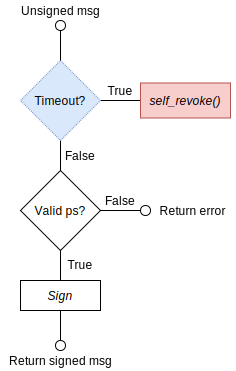
\includegraphics[width=\columnwidth]{figures/drawio/flowchart-sign.drawio.pdf}
    \end{subfigure}
    \unskip\ \vrule\
    \begin{subfigure}[T]{.4\columnwidth}
        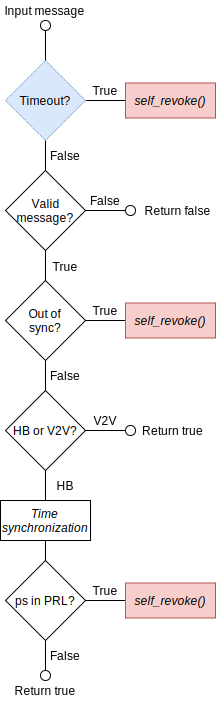
\includegraphics[width=\columnwidth]{figures/drawio/flowchart-process.drawio.pdf}
    \end{subfigure}
    \begin{minipage}{.45\columnwidth}
        \leavevmode\subcaption{Receiving a sign request.}
        \label{fig:appendix:flowchart-sign}
    \end{minipage}\hfil
    \begin{minipage}{.45\columnwidth}
        \leavevmode\subcaption{Receiving a message.}
        \label{fig:appendix:flowchart-process}
    \end{minipage}
    \caption{Flowcharts of the \acs{TC} logic. Blue (dotted) nodes are only
    relevant when a local trusted time source is available in \acsp{TC}.}
    \label{fig:appendix:flowchart}
\end{figure}

%Table~\ref{tbl:eval-variables} describes all variables used in the main paper
%for the reader's convenience. 
\cref{fig:appendix:flowchart} depicts flowcharts for the \ac{TC} behavior
described in our design. In particular, \cref{fig:appendix:flowchart-sign}
illustrates the steps taken to sign a \ac{V2V} message, while
\cref{fig:appendix:flowchart-process} shows the logic to verify a network
message, which can be either a \ac{HB} or a \ac{V2V} message.

According to \cref{req:v2v-receive,eq:valid-v2v-generic,eq:valid-heartbeat},
external messages should be verified with respect to authenticity (via digital
signature verification) and freshness (according to the validity window
\paramtt). Furthermore, the \ac{TC} should automatically perform self-revocation
if it detects de-synchronization (\cref{eq:auto-rev}). For every valid \ac{HB},
the \ac{TC} should synchronize its internal time \funcnow{}
((\cref{eq:time-update}), redundant if a local trusted time source is used), and
then inspect the \ac{PRL} to check whether self-revocation should be executed or
not (\cref{eq:self-rev}). For signing a message, the \ac{TC} should possess
valid pseudonyms in order to make a signature, which includes the input message
and context metadata such as timestamps (\cref{req:v2v-send}).

In \cref{fig:appendix:flowchart}, the \emph{timeout} condition in blue only
applies to the extension that takes into account a local trusted time source in
\ac{TC}, and checks if the current time is bigger than the biggest timestamp
received in a \ac{HB} plus \paramtt{} (\cref{eq:auto-rev-timeout}).
\section{Tamarin Models}
\label{appendix:tamarin}

This appendix extends \cref{section:design-verification}, providing more details
on how we translated our design to \tamarin{} and how we captured the properties
of our design. Here, we also discuss our variant where a trusted time source in
the \ac{TC} is available (cf.~\cref{section:design-extensions}).

\subsection{Mapping our Design to \tamarin{}}

To map our design to Tamarin, we used only six main rules:
%
\begin{itemize}
    \item \tamrule{RA\_generate\_heartbeat}: This rule takes as input the
    current time and \ac{PRL} and produces a new \ac{HB} as output, signed
    with the \ac{RA}'s private key. The \ac{HB} is also sent out to the network
    channel, and an action fact \tamrule{HeartbeatGenerated(HB)} is produced.
    This rule can only be executed once per \ac{PRL} and time step to reduce
    the number of states, since multiple execution with the same parameters
    would generate the same \ac{HB}, which is not relevant in our model since
    \tamarin{} already allows replays of network messages.
    \item \tamrule{RA\_issue\_revocation}: Taking as input the current
    time, \ac{PRL}, and a pseudonym's public key, this rule generates a
    new \ac{PRL} by adding the pseudonym to the list and incrementing the
    sequence number by one. We added a restriction to revoke each pseudonym only
    once. After execution, the action fact \tamrule{RevocationIssued(ps, t)} is
    generated.
    \item \tamrule{TC\_get\_pseudonym}: This rule allows the \ac{TC} to obtain a
    new pseudonym credential. How exactly this credential is obtained (e.g., via
    a communication to the infrastructure) is outside of our scope; What is
    important in our model is that the \ac{TC} can obtain and use an arbitrary
    number of pseudonyms. The only restriction of this rule is to ensure that
    only non-revoked \acp{TC} can obtain new pseudonyms
    (cf.~\cref{req:pseudonym}).
    \item \tamrule{TC\_process\_heartbeat}: The \ac{TC} processes a \ac{HB}
    taken as input from the channel. Restrictions ensure that the received
    \ac{HB} has a valid signature and timestamp. In addition, the \ac{TC} has to
    check whether to perform self-revocation or not. To do so, we divided this
    rule in two mutually-exclusive rules that produce different results: if any
    of the \ac{TC} pseudonyms is in the \ac{PRL}, the action fact
    \tamrule{Revoked(t)} is produced, otherwise it is not. Either way, a
    \tamrule{HeartbeatProcessed(HB,t)} action fact are produced, along with a
    new \tamrule{!Time(t\_hb)} persistent fact to synchronize the \ac{TC} time.
    \item \tamrule{TC\_sign\_message}: The \ac{TC} generates a new \ac{V2V}
    message signed with a pseudonym's private key. It takes the latest time as
    input, while restrictions ensure that the TC has not been previously revoked
    (i.e., the \tamrule{Revoked(t)} action fact does not exist). The rule
    produces a signed timestamped message and sends it to the out channel. A
    \tamrule{Signed(msg,ps)} action fact is produced as well.
    \item \tamrule{process\_message}: This rule models a generic third entity
    that receives a \ac{V2V} message from network and verifies it. If the
    signature is valid and the message is fresh, a
    \tamrule{MessageAccepted(msg,ps,t)} action fact is generated.
\end{itemize}

\subsection{Trusted Time Source in \acp{TC}}

\begin{figure}
  \centering
    \lstinputlisting[language=Tamarin]{properties-time.spthy}
  \caption{Properties of our design with a trusted time source in \ac{TC}
  translated to \tamarin{} lemmas.}
  \label{listing:tamarin-lemmas-time}
\end{figure}

The design that models a trusted time source in \ac{TC} comes with a major
difference, i.e., that \ac{TC} and \ac{RA} use the same \tamrule{!Time} facts.
That is, this means that their clock is perfectly synchronized, and the \ac{TC}
does not need to process \acp{HB} to advance its internal time.

Table~\ref{tbl:tamarin-lemmas-trusted-time} provides the full list of lemmas
used in this variant, most of which are analogous to the main model. The main
difference is that we added three \emph{reusable lemmas}, i.e., lemmas that
\tamarin{} can leverage to prove other lemmas. This was helpful since we
experienced that the two proof lemmas were harder to verify efficiently than in
our main model. By defining additional lemmas marked as \tamrule{reuse}, we
could instead build efficient proofs, allowing \tamarin{} to terminate in only a
few minutes.


\cref{listing:tamarin-lemmas-time} shows the proof properties of this model. Two
are the main differences compared to the main model: First, the
\tamrule{effective\_revocation} lemma can now directly prove our first property
to calculate the exact value for \paramteff. Indeed, we now assume that all
\acp{TC} are perfectly synchronized with the \ac{RA} time, hence the revocation
time is now absolute and comes at $\paramtrev + 2\paramtt$. Second, thanks to
internal timeouts in \ac{TC}, we can have a stronger proof for the second
property, saying that not only does the \ac{TC} not process \acp{HB} generated
after $\paramtrev{} + \paramtt{}$, but also that the \ac{TC} cannot perform
\emph{any} operations after that time because the automatic revocation timeout
would be triggered. To prove this, we defined an additional rule called
\tamrule{TC\_do\_operation}, which models a generic operation performed by the
\ac{TC} via the \tamrule{NewOperation(t)} action fact. This is then used in
\tamrule{no\_operations\_after\_timeout} to prove that there cannot be
\tamrule{NewOperation(t)} action facts with a value for $t$ bigger than
$\paramtrev + \paramtt$.

\begin{table*}
    \renewcommand{\arraystretch}{1.2}
    \newcolumntype{L}{>{\raggedright\arraybackslash}X}
      \centering
      \begin{tabularx}{.97\linewidth}{ | l | c | c | c | L | }
        \hline
        Lemma                                                     & Type   &  Oracle      & Steps & Description  \\
        \hline
        \hline
        \tamrule{sign\_possible}                                  & S      &              & 6     & Ensures that the \ac{TC} can sign \ac{V2V} messages \\
        \hline
        \tamrule{generate\_hb\_possible}                          & S      &              & 5     & Ensures that the \ac{RA} can generate and distribute \acp{HB} \\
        \hline
        \tamrule{issue\_revocation\_possible}                     & S      &              & 5     & Ensures that the \ac{RA} can revoke pseudonyms, adding them to the \ac{PRL} \\
        \hline
        \tamrule{processing\_hb\_possible}                        & S      &              & 9     & Ensures that the \ac{TC} can receive and process a \ac{HB} \\
        \hline
        \tamrule{revocation\_possible}                            & S      &              & 13    & Ensures that the \ac{TC} can self-revoke when receiving a \ac{HB} \\
        \hline
        \tamrule{process\_message\_possible}                      & S      &              & 7     & Ensures that a third entity can process \ac{V2V} messages signed by the \ac{TC}  \\
        \hline
        \tamrule{exists\_par\_tv\_2}                              & S      &              & 5     & Used to verify that \paramtt{} is arbitrary \\
        \hline
        \tamrule{exists\_par\_tv\_4}                              & S      &              & 7     & Used to verify that \paramtt{} is arbitrary \\
        \hline
        \tamrule{no\_signing\_after\_timeout}                     & F      &              & 205   & Ensures that the \ac{TC} cannot make signatures after performing automatic revocation \\
        \hline
        \tamrule{no\_signing\_after\_revocation}                  & F      &              & 2     & Ensures that the \ac{TC} cannot make signatures after performing self-revocation \\
        \hline
        \tamrule{all\_heartbeats\_processed\_within\_tolerance}   & F      & \faCheck     & 260   & Ensures that outdated \ac{HB} are correctly discarded by the \ac{TC} \\
        \hline
        \tamrule{all\_messages\_accepted\_signed\_exists}         & R      & \faCheck     & 62    & Ensures that, for each \ac{V2V} message verified by a third entity, the same message was previously signed by the \ac{TC} \\
        \hline
        \tamrule{all\_messages\_accepted\_within\_tolerance}      & R      & \faCheck     & 282   & Ensures that outdated \ac{V2V} messages are correctly discarded by the third entity \\
        \hline
        \tamrule{no\_messages\_accepted\_after\_revocation}       & R      & \faCheck     & 74    & Ensures that, if revocation is mandated at time \paramtrev, all TC messages accepted by a third entity cannot contain timestamp greater than $\paramtrev{} + \paramtt{}$ \\
        \hline
        \tamrule{effective\_revocation}                           & P      & \faCheck     & 4     & Verifies property \ref{property:revoke} in \cref{section:design-properties} \\
        \hline
        \tamrule{no\_operations\_after\_timeout}                  & P      & \faCheck     & 76    & Verifies property \ref{property:prl} in \cref{section:design-properties} \\
        \hline
      \end{tabularx}
      \vspace{0.2cm}
      \caption{Full list of lemmas proven with \tamarin{} on our model with
      trusted time. \emph{Type} is either \emph{S} (sanity), \emph{F}
      (functional), \emph{R} (reuse) or \emph{P} (proof). \emph{Oracle}
      indicates whether an oracle was needed, while \emph{Steps} the number of
      steps required by \tamarin{} to prove the lemma.}
      \label{tbl:tamarin-lemmas-trusted-time}
      %\vspace{-5mm}
    \end{table*}
    %



%\section{Complete Simulation Results}
\label{appendix:simulation}

\begin{table}
\renewcommand{\arraystretch}{1.2}
  \centering
  \begin{tabular}{ | c | c | c | c | c | }
    \hline
    Scenario        & Time? &  \paramtt{} (s)   & \paramteff{} (s)   & \paramtprl{} (s)  \\
    \hline
    \hline
    A1              & no                  & 30                & 60                 & 30                \\
    \hline
    A2              & no                  & 150               & 300                & 150               \\
    \hline
    B1              & yes                 & 30                & 60                 & 30                \\
    \hline
    B2              & yes                 & 150               & 300                & 150               \\
    \hline
  \end{tabular}
  \vspace{0.2cm}
  \caption{ Scenarios evaluated in our simulation. Parameters are chosen
  according to the desired \paramteff{}. The column named \emph{Time?} indicates
  whether a local trusted time source is used in \acp{TC} or not.}
  \label{tbl:eval-scenarios}
  %\vspace{-5mm}
\end{table}
%




\begin{figure}[t]
    %\centering
    \hspace*{-0.3cm}
    \resizebox{1.05\linewidth}{!} {
      \input{figures/eval-simulation.tex}
    } \caption{Simulation results for scenario A1.}
    \label{fig:eval-sim-a1}
\end{figure}

\begin{figure}[t]
    %\centering
    \hspace*{-0.3cm}
    \resizebox{1.05\linewidth}{!} {
      \input{figures/appendix-sim-a2.tex}
    } \caption{Simulation results for scenario A2.}
    \label{fig:eval-sim-a2}
\end{figure}

\begin{figure}[t]
    %\centering
    \hspace*{-0.3cm}
    \resizebox{1.05\linewidth}{!} {
      \input{figures/appendix-sim-b1.tex}
    } \caption{Simulation results for scenario B1.}
    \label{fig:eval-sim-b1}
\end{figure}

\begin{figure}[t]
    %\centering
    \hspace*{-0.3cm}
    \resizebox{1.05\linewidth}{!} {
      \input{figures/appendix-sim-b2.tex}
    } \caption{Simulation results for scenario B2.}
    \label{fig:eval-sim-b2}
\end{figure}

We ran simulations for each of the scenarios described in
\cref{tbl:eval-scenarios}. Results are depicted in
\cref{fig:eval-sim-a1,fig:eval-sim-a2,fig:eval-sim-b1,fig:eval-sim-b2}.

Recall from \cref{section:eval-sim} that each value of the boxes represents the
time between the revocation of \ps{} (\funcrevokedaa{} event) and the last
\ac{V2V} message signed with \ps{} that was verified by a non-malicious \ac{TC}
(\funcverify{} event). The latter time represents the \emph{effective revocation
time} for that particular pseudonym \ps. The box plots give the distribution of
such values, obtained aggregating more than 600 revocations, filtering out
negative values.

The figures show one significant difference between the main design (A1 and A2)
and the extension with a local trusted time source (B1 and B2): While in the
former most revocations are effective around or before \paramtt{}, in the latter
attackers are able to postpone revocation up until \paramteff{} in some cases,
i.e., it appears easier to reach the upper bound, especially for powerful
attackers such as the \attackersmart{} one. This is due to the fact that, while
in the main design revoked \acp{TC} cannot synchronize their time since
\paramtrev, with a local time source \acp{TC} can still advance their internal
time up until $\paramtrev + \paramtt$, before triggering the automatic
revocation logic. That is, in the latter case a revoked \ac{TC} is able to
generate ''more fresh'' \ac{V2V} messages, which can be processed by other
\acp{TC} later in time.

This peculiarity suggests that a local trusted time source negatively affects
the revocation time. While this may be true in the average case, it still does
not affect the worst-case effective revocation time \paramteff, as shown in the
figures.
\section{Calculating Expected Size of the PRL}
\label{appendix:markov}

This appendix covers the basics of the utilized probabilities to then explain
the Markov matrix. We also describe the calculation of the stationary
distribution as a means to calculate the expected \ac{PRL} size. Finally, we
discuss the computation of the probabilities and expected values used in
\cref{section:eval-prl-size}.

\subsection{Utilized Probabilities}

Recall from \cref{section:eval-prl-size} that we model the processes of gaining
and losing pseudonyms from the \ac{PRL} as two individual probabilities, then we
combine them in the next step into a Markov chain. The two probabilities shown
in \cref{eq:prl-size-g} and \cref{eq:prl-size-l} are denoted as $G_{il}$ and
$L_{il}$ respectively and can be seen as probability matrices that at location
$il$ have the probability for being in state $i$ and gaining or losing $l$
pseudonyms from the list. The core assumption for these two probabilities is
that both adding and removing pseudonyms from the revocation list can be seen as
a binomial distribution that only depends on:
\begin{inparaenum}
    \item the current size of the list, i.e., how many certificates there are left to be revoked or removed from the list,
    \item the probability for each pseudonym to be revoked at any given time, and
    \item the time that a pseudonym stays in the list.
\end{inparaenum}
As such, this model assumes that pseudonyms are renewed as soon as they are
evicted from the \ac{PRL}, i.e., the list can never hold more than the total
number of $n$ pseudonyms, which is a realistic assumption for large $n$ as it is
unlikely that so many pseudonyms in the system would be revoked in a short time
during regular operation.  Furthermore, in this way we model the process of
losing pseudonyms from the list as a probabilistic process that has the expected
value at $T_{prl}$.  We, however, can not model a precise eviction of the
pseudonym from the \ac{PRL} after $T_{prl}$ time steps.  In our view this is an
acceptable tradeoff as on average and over the lifetime of the \ac{PRL}, the
modeled behavior comes very close to the actual behavior of evicting pseudonyms
from the \ac{PRL} after exactly $T_{prl}$ time steps.

\subsection{Markov Model}
We can now combine these two probabilities into a matrix that at location
$p_{ij}$ has the probability of moving from state $i$ to state $j$. Starting
with the simple example of $n=3$ pseudonyms, multiple entries of this matrix are
straightforward:
\begin{itemize}
    \item Starting at any state $i$ and stepping into state $j=0$ requires to not revoke any new pseudonyms and to lose all existing pseudonyms from the list. This is the combination of the two probabilities $L_{ii}G_{i0}$. For example, going from state $i=2$ to $j=0$ requires to lose 2 pseudonyms when there are $2$ in the \ac{PRL}, and requires to gain no new pseudonyms when there are already $2$, leading to the two probabilities $L_{22}G_{20}$
    \item Starting at state $i=0$ and stepping into a state $j$ implies that no pseudonyms can be lost from the \ac{PRL} and $j$ pseudonyms have to be added.
    \item Similarly, starting in state $i=3$ and stepping into any state $j$
    implies that no pseudonyms can be gained, but $j-i$ pseudonyms are removed
    from the \ac{PRL}.
\end{itemize}

The most interesting state transitions in this probability matrix are the
transitions that consist of multiple combinations of events. One example is the
transition from $i=2$ to $j=1$. Here, we first have the obvious possibility that
we reach the state $j=1$, i.e., one pseudonym in the \ac{PRL}, by losing one
pseudonym and gaining none. However, we also have the possibility to lose both
pseudonyms in the \ac{PRL} and gain one, leading to still one remaining
pseudonym in the \ac{PRL}. This is because the pseudonyms in the \ac{PRL} and
outside of the \ac{PRL} are independent and pseudonyms can still be revoked
while others are removed from the list. Thus, the state transition consists of
the following parts: $p_{21} = L_{21}G_{20} + L_{22}G_{21}$.

The full state probability matrix for $n=3$ pseudonyms can be seen below. Note
that a matrix for $n$ pseudonyms is a $n+1 \times n+1$ matrix to accommodate the
state of the empty \ac{PRL}.\vspace{2mm}\\
\begin{math}
    P =
    \left[ {\begin{smallmatrix}{}
      L_{00}G_{00} & L_{00}G_{01} & L_{00}G_{02} & L_{00}G_{03} \\
      L_{11}G_{10} & L_{10}G_{10} + L_{11}G_{11} & L_{10}G_{11} + L_{11}G_{12} & L_{10}G_{12} \\
      L_{22}G_{20} & L_{21}G_{20} + L_{22}G_{21} & L_{20}G_{20} + L_{21}G_{21} & L_{20}G_{21} \\
      L_{33}G_{30} & L_{32}G_{30} & L_{31}G_{30} & L_{30}G_{30} \\
    \end{smallmatrix} } \right]
\end{math}
\vspace{2mm}

\begin{figure}
    \centering
    \includegraphics[width=.85\columnwidth]{figures/markov-tikzplot/small-tikz.pdf}
    \caption{A graph of the Markov chain with the exemplary parameters of $n=3$, $p=0.1$, and $T_{prl}=2$.}
    \label{fig:appendix:markov-graph}
\end{figure}

Such probability matrices are also called discrete time Markov
chains~\cite{hermanns2002markov}. \Cref{fig:appendix:markov-graph} depicts the
transition graph for the above Markov chain when we assume the parameters of
$p=0.1$ and $T_{prl}=2$. Based on this first small example, we can approach a
closed formula for an arbitrary number of pseudonyms ($n$). This closed formula
is shown in \cref{eq:prl-size-markov}. The core idea is that each entry depends
on a combination of gaining and losing pseudonyms based on the maximum of $i-j$
and $0$ and ranges up to $i$. Then, any state combination that is not possible
will be $0$ through the binomial coefficient. However, this range is necessary
to catch the complicated combinations in the center of the matrix. Each
combination is then based on losing $l$ pseudonyms from the list and gaining
$l-i+j$ pseudonyms, which basically iterates through the combinations with $l$
as a stepping variable.

\subsection{Calculating the Expected PRL Size}

In discrete time Markov chains, a probability state vector $\pi$ can be multiplied with the Markov matrix $P$ to gain the probabilities for $\pi$ after a single transition in the model~\cite{hermanns2002markov} as follows: $\pi' = \pi \cdot P$.
This, however, is only sufficient to gain the state probabilities after specific amounts of steps.
In contrast to this approach, Markov chains may approach a so-called state equilibrium which is a stationary probability distribution that does not change even after taking a step in the Markov chain.
The stationary distribution follows the equation $\pi = \pi \cdot P$~\cite{hermanns2002markov}.

To gain this stationary distribution, we solve the following equation system:
\begin{flalign*}
                &\pi = \pi P&\\
&\leftrightarrow \pi - \pi P = 0&\\
&\leftrightarrow \pi ( I - P ) = 0&\\
&\leftrightarrow ( I - P )^T \pi^T = 0&
\end{flalign*}

Lastly, since there may be several solutions to this linear equation, we add the
specific constraint to this equation system that the sum of $\pi$ is equal to
$1$. This is the case for each probability vector in Markov
models~\cite{hermanns2002markov}, and follows the intuition that, from any state
probability, the probability to reach any other state is $1$. To add this
constraint, we add a row of $1$ to $( I - P )^T$ and append a $1$ to the zero
vector. Solving this linear equation yields a stationary distribution that is
stable. \cref{fig:eval-prl-size} summarizes this stationary distribution by
showing the list sizes that occur to 75\%, 90\%, and to 99.99\%. The graph shows
these percentiles under different scenarios, i.e., with different shares of
attackers in the network.

\begin{figure}[t]
    \centering
    \resizebox{.83\linewidth}{!}{% changed from auto generated plot:
% width=\columnwidth,
% legend pos=north west,
% and escape the % signs in the labels
% Color order: steelblue88116163 peru20313699 mediumseagreen95157109 indianred1819295
% This file was created with tikzplotlib v0.10.1.
\begin{tikzpicture}

\definecolor{lightgray204}{RGB}{204,204,204}
\definecolor{darkslategray38}{RGB}{38,38,38}
\definecolor{darkslategray76}{RGB}{76,76,76}
\definecolor{indianred1819295}{RGB}{181,92,95}
\definecolor{lavender234234242}{RGB}{234,234,242}
\definecolor{lightslategray133122170}{RGB}{133,122,170}
\definecolor{mediumseagreen95157109}{RGB}{95,157,109}
\definecolor{peru20313699}{RGB}{203,136,99}
\definecolor{steelblue76114176}{RGB}{76,114,176}
\definecolor{steelblue88116163}{RGB}{88,116,163}


\begin{axis}[
width=\columnwidth,
legend pos=north west,
ylabel= PRL size (99th percentile),
xlabel= Number of pseudonyms,
xmajorgrids,
xmajorticks=true,
ymajorgrids,
ymajorticks=true,
axis background/.style={fill=lavender234234242},
axis line style={white},
x grid style={white},
y grid style={white},
legend cell align={left},
legend style={
fill opacity=0.8,
draw opacity=1,
text opacity=1,
at={(0.03,0.97)},
anchor=north west,
draw=lightgray204,
% fill=lavender234234242
},
tick align=outside,
tick pos=left,
xmin=370, xmax=1030,
xtick style={color=black},
ymin=0.0, ymax=15.5,
ytick style={color=black}
]
\addplot [draw=steelblue88116163, fill=steelblue88116163, mark=*, only marks]
table
\addplot [draw=peru20313699, fill=peru20313699, mark=triangle*, only marks]
table
\addplot [draw=mediumseagreen95157109, fill=mediumseagreen95157109, mark=square*, only marks]
table
\addplot [draw=indianred1819295, fill=indianred1819295, mark=diamond*, only marks]
table
\end{axis}

\end{tikzpicture}} 
    \caption{99th percentile PRL sizes for fixed $T_{prl}=30$ and varying number of pseudonyms ($n$) under four scenarios.}
    \label{fig:appendix:markov-n}   
\end{figure}

\begin{figure}[t]
    \centering
    \resizebox{.83\linewidth}{!}{% changed from auto generated plot:
% width=\columnwidth,
% legend pos=north west,
% and escape the % signs in the labels
% Color order: steelblue88116163 peru20313699 mediumseagreen95157109 indianred1819295

% This file was created with tikzplotlib v0.10.1.
\begin{tikzpicture}

\definecolor{lightgray204}{RGB}{204,204,204}
\definecolor{darkslategray38}{RGB}{38,38,38}
\definecolor{darkslategray76}{RGB}{76,76,76}
\definecolor{indianred1819295}{RGB}{181,92,95}
\definecolor{lavender234234242}{RGB}{234,234,242}
\definecolor{lightslategray133122170}{RGB}{133,122,170}
\definecolor{mediumseagreen95157109}{RGB}{95,157,109}
\definecolor{peru20313699}{RGB}{203,136,99}
\definecolor{steelblue76114176}{RGB}{76,114,176}
\definecolor{steelblue88116163}{RGB}{88,116,163}

\begin{axis}[
width=\columnwidth,
legend pos=north west,
ylabel= PRL size (99th percentile),
xlabel= $T_{prl}$,
xmajorgrids,
xmajorticks=true,
ymajorgrids,
ymajorticks=true,
axis background/.style={fill=lavender234234242},
axis line style={white},
x grid style={white},
y grid style={white},
legend cell align={left},
legend style={
fill opacity=0.8,
draw opacity=1,
text opacity=1,
at={(0.03,0.97)},
anchor=north west,
draw=lightgray204
},
tick align=outside,
tick pos=left,
x grid style={white},
xmin=5, xmax=205,
xtick style={color=black},
y grid style={white},
ymin=0.0, ymax=52,
ytick style={color=black}
]
\addplot [draw=steelblue88116163, fill=steelblue88116163, mark=*, only marks]
table
\addplot [draw=peru20313699, fill=peru20313699, mark=triangle*, only marks]
table
\addplot [draw=mediumseagreen95157109, fill=mediumseagreen95157109, mark=square*, only marks]
table
\addplot [draw=indianred1819295, fill=indianred1819295, mark=diamond*, only marks]
table
\end{axis}

\end{tikzpicture}
} 
    \caption{99th percentile PRL sizes for fixed $n=800$ pseudonyms and varying $T_{prl}$ under four scenarios.}
    \label{fig:appendix:markov-e}  
\end{figure}

In the following, we expand this evaluation with Figures
\ref{fig:appendix:markov-n} and \ref{fig:appendix:markov-e}.
\Cref{fig:appendix:markov-n} depicts only the 99th percentile for a fixed
$T_{prl}$ and only focuses on the four extreme cases: For each of the two
baseline scenarios, 0\% and 20\% of attackers in the network. The horizontal
axis then depicts a growing number of pseudonyms (and, therefore, vehicles) in
the network. This is to show that a larger number of vehicles does not
exponentially grow the expected size of the \ac{PRL}. Instead, the 99th
percentile of the list size grows linearly with $n$. Similarly,
\cref{fig:appendix:markov-e} shows the same situation for a fixed number of
pseudonyms at $n=800$ but a varying window for $T_{prl}$. This second graph
shows that the \ac{PRL} size also grows linearly with a linear increase in the
time that a pseudonym stays in the \ac{PRL}.

\subsection{Probabilities and Expected Revocations}

Above, $p$ is the probability of revocation in each time step. As time steps are at the granularity of seconds, and our system runs for a long time, it turns out that the per-step probabilities leading to realistic revocation rates are very small. Instead, the probabilities used in the \ac{PRL} size evaluation were described in terms of a compound probability $q$ that a revocation occurs at least once over a number of $s$ steps. This probability can be computed via the geometric series
\[q(p,s) = \sum_{i=1}^s p\cdot(1-p)^{i-1} = 1-(1-p)^s\] 
which sums up the probabilities that the first revocation occurs the first time in step $i\in[1:s]$. Note that this is equal to $1$ minus the probability that in all $s$ steps no revocation occurs. Solving for $p$ we obtain
\[p(q,s) = 1-\sqrt[s]{1-q}\,.\]
We used this formula to compute the baseline per-step probabilities underlying our scenarios for honest vehicle and attacker separately. The final probabilities $p$ for the Markov models were then obtained by averaging the probabilities weighted according to the share of attackers.

For estimating the expected numbers of revocations in our scenarios we needed to calculate the expected value for $n$ pseudonyms over $s$ steps. If each step was independent this would simply be $n\cdot s \cdot p$, however, as explained above, in our Markov model at most $n$ pseudonyms can be revoked at a time. We compensated for this fact by taking into account the chance $p_{\mathrm{prl}}$ that a given pseudonym is on the \ac{PRL} at any given time and computed the desired estimate $E_{\mathrm{rev}}$:
\[ E_{\mathrm{rev}}=n\cdot s \cdot p \cdot (1-p_{\mathrm{prl}}) \]
We set $p_{\mathrm{prl}}$ to the median \ac{PRL} size, as obtained by the Markov model for each scenario, divided by $n$.

\section{Artifact Appendix}

This Appendix contains a complete description on the artifacts presented in our
paper, along with detailed instructions for running the artifacts locally and
reproducing our results.

\subsection{Description \& Requirements}
\label{artifact:requirements}

\begin{table}
\renewcommand{\arraystretch}{1.2}
  \centering
  \begin{tabular}{ | c | c | }
    \hline
    Software                    & Tested version                            \\
    \hline
    \hline
    Docker                      & 23.0.2                                    \\
    \hline
    Docker Compose              & 2.17.2                                    \\
    \hline
    kubectl                     & 1.28.2                                    \\
    \hline
    Minikube                    & 1.31.2 (running Kubernetes 1.27.4)        \\
    \hline
  \end{tabular}
  \vspace{0.2cm}
  \caption{List of all software dependencies required to run our artifacts, along with the version that we used in our setup.}
  \label{tbl:artifact-sw}
  %\vspace{-5mm}
\end{table}
%




This section provides all the information necessary to recreate the experimental
setup to run our artifacts. All experiments can run on a commodity desktop
machine. For experiment (E2), we provide a scaled-down configuration that can
still provide meaningful results. See \cref{artifact:evaluation} for more
details.

\subsubsection{How to access}
The artifacts are publicly available on Github\footnote{\repo{}}. While the
\texttt{main} branch contains the latest version of the code, the
\texttt{ndss-24-artifacts} tag contains the exact version of the code that was
submitted for review in the artifact evaluation. The latter is also available on
Zenodo~\cite{supplMaterial}.

\subsubsection{Hardware dependencies}
Our artifacts can be run on a commodity desktop machine with a x86-64 CPU. To
ensure that all artifacts run correctly, it is recommended to use a machine with
at least 8 cores and 16 GB of RAM.

\subsubsection{Software dependencies} 
A recent Linux operating system is required, preferably one between Ubuntu
$\geq$ 20.04 and Debian $\geq$ 10. Our artifacts have been tested on Ubuntu
22.04 LTS (Jammy). Additional dependencies are listed in \cref{tbl:artifact-sw}.

\subsubsection{Benchmarks} 
None.

\subsection{Artifact Installation \& Configuration}
\label{artifact:configuration}

We first require that our repository is downloaded to a local folder, e.g., via
\texttt{git clone}. To install all required dependencies, we then provide an
\texttt{install.sh} script that can be used by Ubuntu and Debian users to
install up-to-date versions of the packages listed in \cref{tbl:artifact-sw}.
Alternatively, such dependencies can be installed manually via official
channels. Note that we require running the installation script and subsequent
experiments using a non-root user with \texttt{sudo} privileges.

All artifacts leverage Docker containers for ease of use. However, except for
experiment (E2), all experiments can be run locally. Additionally, most
experiments have customizable parameters. In this Appendix, we provide
instructions for running all experiments with Docker using a fixed set of
parameters, but our repository contains extensive instructions for customizing
each experiment.

\subsection{Experiment Workflow}

Our artifacts contain three independent experiments. The first consists in the
formal verification of our design using the Tamarin prover. The second
experiment simulates a \ac{V2X} scenario on Kubernetes, where our scheme is
evaluated under different conditions. The third experiment performs a
statistical evaluation on the size of \ac{PRL} to assess the scalability of our
approach.

The proposed workflow runs the three experiments sequentially. Our repository
contains scripts and a Makefile that can be used to automate all experiments.
For brevity, this Appendix only illustrates the \texttt{make} commands to run at
each step, while extensive documentation is provided in our repository.

\subsection{Major Claims}

\begin{itemize}
    \item (C1): Our scheme guarantees revocation within a deterministic upper
    bound \paramteff, even in case of delayed or dropped revocation requests.
    This is proven by experiment (E1), whose results are reported in
    \cref{section:design-verification}, Appendix~\ref{appendix:tamarin} and
    \cref{tbl:tamarin-lemmas-main,tbl:tamarin-lemmas-trusted-time}.
    \item (C2): Our scheme is resilient to severe network malfunctions and
    delays that may occur in a real-world scenario. Even in these harsh
    conditions, revocation times are not only within the upper bound proven in
    C1, but also significantly shorter on average. This is proven by experiment
    (E2), whose results are reported in \cref{section:eval-sim} and
    \cref{fig:eval-sim-base}. Additional experiments are described in our Github
    repository.
    \item (C3): Our scheme scales well with the number of vehicles and attackers
    in the network. Additionally, even when choosing a small \paramteff{}, the
    required network and computational resources are still low. This is proven
    by experiment (E3), whose results are reported in
    \cref{section:eval-prl-size}, Appendix~\ref{appendix:markov} and
    \cref{fig:eval-prl-size,fig:eval-tv,fig:appendix:markov-e,fig:appendix:markov-n}.
\end{itemize}

\subsection{Evaluation}
\label{artifact:evaluation}

This section includes all the operational steps and experiments which must be
performed to evaluate our artifacts and validate our results. In total, all
experiments require between 30 and 60 human-minutes and around 8 compute-hours.
We assume that the machine is configured correctly with required dependencies,
as described in \cref{artifact:requirements,artifact:configuration}. The same
instructions, along with additional details, are provided in the top-level
README file of our repository.

\subsubsection{Experiment (E1) - Claim (C1)}
\label{artifact:proofs}
[Tamarin proofs] [2 human-minutes + 10 compute-minutes]: The experiment consists
in using the open-source Tamarin prover tool (version 1.6.1\footnote{The
recently-released version of Tamarin 1.8.0 is not able to verify our models
efficiently. We are currently investigating this issue.}) to verify our
revocation design. Tamarin receives as input our model specification along with
the properties (\textit{lemmas}) we want to verify, and attempts to verify such
properties. Our artifacts include two separate models, one that illustrates the
main design in \cref{chapter:design} and another that illustrates a variation of
our design where \acs{TC} have a trusted time that is synchronized with the
\acs{RA} (\cref{section:design-extensions}). See
\cref{section:design-verification} and Appendix~\ref{appendix:tamarin} for more
information.

\textit{[Preparation]} In a new shell, go to the \texttt{proofs} folder.

\textit{[Execution]} Firstly, prove the main design, which is called
\texttt{centralized-time}. The command to run, along with the expected output,
is provided below.

\begin{lstlisting}[language=bash]
# Prove the `centralized-time` model (5 minutes)
# Expected output: 
# - Tamarin prints a "summary of summaries" at the end
# - In the summary, all lemmas are marked as "verified"
# - a `output_centralized.spthy` file under `./out`
make prove MODEL=centralized-time OUT_FILE=output_centralized.spthy
\end{lstlisting}

Secondly, prove the variation of our design with trusted time, which is called
\texttt{distributed-time}. The command to run, along with the expected output,
is provided below.

\begin{lstlisting}[language=bash]
# Prove the `distributed-time` model (5 minutes)
# Expected output: 
# - Tamarin prints a "summary of summaries" at the end
# - In the summary, all lemmas are marked as "verified"
# - a `output_distributed.spthy` file under `./out`
make prove MODEL=distributed-time OUT_FILE=output_distributed.spthy
\end{lstlisting}
    
\textit{[Results]} Upon completion, Tamarin prints to standard output a summary
where each lemma is marked either as \emph{verified}, \emph{falsified}, or
\emph{analysis incomplete}. In our case, the experiment can be considered
successful if all lemmas are marked as \emph{verified}. The output files
\emph{output\_\{centralized,distributed\}.spthy}, contain the full proofs
computed by Tamarin.

\subsubsection{Experiment (E2) - Claim (C2)}
\label{artifact:simulations}
[Simulations] [20-30 human-minutes + 4.5-5 compute-hours]: The experiment
consists in simulating a \acs{V2X} edge area with a number of vehicles that
interact with each other, some of them being malicious. The goal of this
simulation is collecting data on revocation times for malicious vehicles, and
analyzing their distribution compared to different scenarios and attacker
levels. See \cref{section:eval-sim} for more information. The simulation runs on
a Kubernetes cluster: Our experiments have been carried out on a large cluster
with 8 nodes, spawning 400 vehicles and with a total simulation time of around
32 hours. For the artifact evaluation, however, we propose a \emph{scaled-down}
configuration that can run locally on a Minikube instance and spawns 50
vehicles, with a total simulation time of around 4 hours. We believe that this
configuration is still acceptable since it only affects the quantity of gathered
data (i.e., number of revocations and revocation times). The output plots will
therefore be comparable to the figures in our paper, although less data will
produce less outliers. Besides, given that there is a certain degree of
randomicity (due to simulated network conditions), it is impossible to reproduce
\emph{exactly} the same results that are shown in the paper: Each simulation,
therefore, will produce slightly different box plots.

\textit{[Preparation]} In a new shell, go to the \texttt{simulation} folder. Run
the commands below in sequence to set up a new Minikube cluster and build our
application.

\begin{lstlisting}[language=bash]
# Create a new Minikube instance (1-5 minutes)
# Expected output:
# - A success message from Minikube
# - kubectl works correctly: try running `kubectl get nodes`
make run_minikube

# Build application from source (3 minutes)
# Expected output: No error messages
make build_minikube
\end{lstlisting}

\textit{[Execution]} To run all simulations at once, run the command below. Our
scripts will autonomously manage each simulation and collect all data.

\begin{lstlisting}[language=bash]
# Run all simulations (4.5-5 hours)
# Expected output:
# - a `simulations` folder created. `simulations/scenarios` contain one file for each run (16 in total)
# - (after 1 minute since start) the log file `simulations/out.log` does not show errors and is "SLEEPING"
# - (after 2-3 minutes since start) `kubectl -n v2x get pods` shows all pods in "Running" state
# - (after 4.5-5 hours since start) the log file `simulations/out.log` shows "ALL DONE" as last message
# - (after 4.5-5 hours since start) the `simulations/results` folder contains one file for each run (16 in total)
make run_simulations_background CONF=conf/ae.yaml
\end{lstlisting}

\textit{[Results]} Assuming that all simulations have been successful, the plots
can be generated by running \texttt{make plot\_all}. The results can be then
found in the \emph{simulations/figs} folder. Scenario A1 corresponds to
\cref{fig:eval-sim-base}, while the other scenarios are described in our Github
repository.

\subsubsection{Experiment (E3) - Claim (C3)}
\label{artifact:prl}
[Size of the \acs{PRL}] [10-20 human-minutes + 2.5-3.5 compute-hours]: The
experiment consists in creating a statistical model for the size of the
\ac{PRL}, where the process of adding and removing pseudonyms can be
approximated to a Markov model. Then, based on this model, we plot the expected
\ac{PRL} sizes in terms of percentiles of all possible states, using different
parameters such as the number of pseudonyms, the time each pseudonym needs to
stay in the \ac{PRL} (\paramtprl{}) and the share of attackers in the network.
See \cref{section:eval-prl-size} and Appendix~\ref{appendix:markov} for more
information.

\textit{[Preparation]} In a new shell, go to the \texttt{prl} folder.

\textit{[Execution]} All the data and plots can be computed with one single
command: \texttt{make all}. Alternatively, each plot can be computed separately
according to the instructions below.

\begin{lstlisting}[language=bash]
# probabilities and expected revocations (1-5 seconds)
# Expected output: results printed to standard output
make probabilities

# Fig. 15: transition graph (1-5 seconds)
# Expected output:
# - no errors printed to standard output
# - `tikz-graph.tex` plot under `./plots`
make tikz

# Fig 6: Series over different probabilities (15-20 min)
# Expected output: 
# - no errors printed to standard output
# - plots `p-plot_n800_e30.{tex,png}` under `./plots`
make p-plot

# Fig. 16: Series over different number of pseudonyms (25-35 min.)
# Expected output:
# - no errors printed to standard output
# - plots `n-plot_e30.{tex,png}` under `./plots`
make n-plot

# Fig. 17: Series over different T_prl (90-140 minutes)
# Expected output:
# - no errors printed to standard output
# - plots `t-plot_n800.{tex,png}` under `./plots`
make t-plot

# Fig. 7: Generate distribution for Tv (15-20 minutes)
# Expected output:
# - no errors printed to standard output
# - plots `tv-distribution.{tex,png}` under `./plots`
make tv-distribution
\end{lstlisting}

\textit{[Results]} Assuming that all commands have succeeded, all plots can be
found in the \emph{plots} folder.


% that's all folks
\end{document}
